\chapter{ مروری بر کارهای گذشته}

\section{مقدمه}
همانطور که در فصل ۱ بیان شد، دو موضوع یافتن چهره \LTRfootnote{Face Detection} در تصویر و شناسایی چهره \LTRfootnote{Face Recognition}، بخش‌های اصلی سامانه تشخیص چهره می‌باشند. اگرچه این دو بخش برای انسان کار ساده ای به نظر می‌رسد، اما برای کامپیوتر‌ها همیشه با چالش همراه بوده است. دلیل این سختی می‌تواند تفاوت تصویرها در مقیاس، حالت چهره، پس زمینه، تابش نور، انسداد و... باشد. در ادامه به بررسی روش‌هایی برای یافتن و شناسایی چهره در دو بخش مجزا پرداخته شده است.
\section{یافتن چهره}
یافتن مکان چهره در تصویر، اولین گام در فرایند تشخیص چهره می‌باشد که نقشی کلیدی در سامانه ایفا می‌نماید. هدف اصلی الگوریتم‌ یافتن چهره این است که تعیین کند آیا چهره ای در تصویر وجود دارد یا خیر و در صورت وجود چهره، مکان آن را بیابد. یافتن چهره در تصویر، امری پیچیده است. زیرا چهره انسان همواره دستخوش تغییراتی مانند شرایط روشنایی و وضوح تصویر، حالت چهره، رنگ پوست، حضور عینک یا موی صورت و... می‌شود. در سال 2002 \lr{Yang} و همکاران \cite{982883} یک دسته بندی برای روش‌های یافتن چهره ارائه کردند که در ادامه شرح داده می‌شود.

\subsection{ رویکردهای مبتنی بر دانش و تطبیق کلیشه}
این رویکردها به مجموعه‌ای از قوانین بستگی دارند و بر اساس دانش انسان در مکان قرار گرفتن اجزای چهره و ویژگی‌های خاصی که در چهره انسان وجود دارد، عمل می‌کنند. یافتن یک جفت چشم در تصویر و سپس جستجو اطراف آن برای یافتن چهره، مثالی از این روش می‌باشد. ابتدا مکان چشم‌ها و بالاترین نقطه سر پیدا می‌شود. سپس فاصله بین چشم تا بالاترین نقطه محاسبه شده و به عنوان یک مرجع برای یافتن نواحی دیگر مانند بینی و دهان مورد استفاده قرار می‌گیرد. این روش زمانی که مو بر روی پیشانی ریخته باشد یا در حضور عینک، به درستی عمل نمی‌کند. یا به عنوان مثالی دیگر، اگر یک توالی از چند فریم در اختیار باشد، می‌توان به کمک اطلاعات حرکت \LTRfootnote{Motion}، یافتن چهره را انجام داد. برای این کار به کمک تفاصل فریم‌ها، قسمت متحرک نسبت به پس زمینه شناسایی شده و بخش بالای آن جدا می‌شود. بدین ترتیب می‌توان با احتمال بالا، مکان چهره یک فرد را در یک تصویر پیدا نمود. این رویکرد در مواجه با اجسام متحرک دیگری مانند اتومبیل دچار اشتباه می‌شود. نمونه های دیگری از این قوانین عبارتند از:

\begin{itemize}
%\setlength\itemsep{0.5em}
\item
هر چهره دارای دو فرو رفتگی برای چشم‌ها است و چیزی شبیه به ابرو روی این فرو رفتگی‌ها قرار دارد.
\item
صورت شامل بینی، چشم‌ها و دهان در فاصله‌ها و موقعیت‌های خاصی با یکدیگر می‌باشد.
\item
چهره مانند یک ناحیه کوچکتر است که بر روی یک ناحیه بزرگتر مانند شانه‌ها قرار گرفته است. 
\item
چهره انسان متقارن است.
\end{itemize} 

\noindent
این رویکردها با استفاده از قالب \LTRfootnote{Template} ‌های از پیش تعیین شده برای یافتن چهره‌ها با همبستگی بین الگوها و تصاویر ورودی استفاده می‌نمایند. چهره انسان را می‌توان به چشم، صورت، بینی و دهان تقسیم کرد. همچنین، با استفاده از روش تشخیص لبه، یک مدل صورت می‌تواند توسط لبه‌ها ساخته شود. این رویکرد ساده است، اما برای تشخیص چهره ناکافی است. با این حال، قالب‌های انعطاف پذیر برای مقابله با این مشکلات پیشنهاد شده‌اند. مشکل بزرگ این رویکرد‌ها، ساختن یک مجموعه مناسب از قوانین است. اگر قوانین خیلی ساده یا خیلی دقیق باشند، الگوریتم همیشه به درستی عمل نمی‌کند. این رویکرد به تنهایی کافی نیست و موفق به یافتن چهره‌ها در شرایط کنترل نشده با تعداد زیادی چهره نمی‌باشد.


\subsection{رویکردهای مبتنی بر ویژگی}
این رویکردها‌ با استخراج ویژگی \LTRfootnote{Feature} ‌های ساختاری چهره، چهره‌ها را پیدا می‌نمایند. ابتدا به عنوان یک طبقه‌بند، آموزش دیده و سپس برای تمایز میان نواحی شامل چهره و بدون چهره در تصویر استفاده می‌شوند. ایده این رویکرد، غلبه بر محدودیت دانش ما از چهره‌ها می‌باشد. در \cite{HJELMAS2001236} تعدادی از این رویکردها مورد بررسی قرار گرفته است:

\subsubsection{رویکرد مبتنی بر لبه}
ابتدا به کمک یک الگوریتم لبه یاب \LTRfootnote{Edge Detection}، لبه‌های تصویر بدست می‌آید، سپس نازک سازی می‌شوند و شاخه‌های اضافه حذف می‌گردد. گوشه لبه‌ها تشخیص داده می‌شوند و هر مولفه متصل \LTRfootnote{Connected Component} به شاخه مرکزی آن کاهش می‌یابد. اجزایی که ویژگی چهره در آن‌ها نیست حذف می‌شوند و اجزای نهایی به عنوان سمت چپ چهره، خط مو، یا سمت راست چهره برچسب گذاری می‌شوند. در یک آزمایش که 60 تصویر دارای پس زمینه پیچیده حاوی 90 چهره به این سامانه داده شده است، سامانه قادر به یافتن 76\% چهره‌ها بوده است.


\subsubsection{رویکرد مبتنی بر اطلاعات سطح خاکستری} 
سطوح خاکستری \LTRfootnote{Gray level} تصویر چهره شامل اطلاعات مفیدی می‌باشد. برای مثال ابرو‌ها، مردمک چشم و لب‌ها معمولا تاریک تر از سایر نواحی صورت هستند. این ویژگی‌ها می‌تواند به یافتن یک چهره در تصویر کمک نماید. در این رویکرد ابتدا بر روی تصویر ورودی، عملیات بسط تباین \LTRfootnote{Contrast Stretching} و عملیات مورفولوژی \LTRfootnote{Morphological Oparations} مبتنی بر سطح خاکستری انجام می‌شود تا تصویر بهبود پیدا کند و یافتن نواحی تیره تر، راحت شود. سپس تصویر به چندین بخش تقسیم می‌شود و سطوح خاکستری بخش‌ها مورد بررسی قرار می‌گیرد. مزیت این رویکرد، کارایی در تصاویر با وضوح پایین می‌باشد (شکل \ref{image2-3}).

\begin{figure}[h]
\centering
  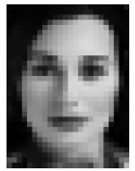
\includegraphics[scale=1]{image2-3}
  \caption{اطلاعات سطح خاکستری حتی در وضوح پایین نیز قابل دسترسی می باشند  \cite{HJELMAS2001236}.}
  \label{image2-3}
\end{figure}

\subsubsection{رویکرد مبتنی بر اطلاعات رنگی}
رنگ در تصویر اطلاعات با ارزشی به ما می‌دهد و می‌توان از رنگ پوست انسان برای یافتن چهره در تصویر استفاده کرد. برای این کار ابتدا رنگ‌ها هنجار سازی \LTRfootnote{Normalization} می‌شوند تا اثر نور پردازی از بین برود. گسترده ترین فضای رنگ مورد استفاده RGB می‌باشد.
\begin{equation}\label{eq2-1}
r = \frac{R}{R + G + B}
\end{equation}

\begin{equation}\label{eq2-2}
g = \frac{G}{R + G + B}
\end{equation}

\begin{equation}\label{eq2-3}
b = \frac{B}{R + G + B}
\end{equation}

در روابط بالا $R$ میزان سطح رنگ قرمز، $G$ میزان سطح رنگ سبز و $B$ میزان سطح رنگ آبی در هر پیکسل از تصویر می‌باشد. همچنین $r$، $g$ و $b$ به ترتیب مقدار هنجار سازی شده برای رنگ قرمز، سبز و آبی می‌باشد. واضح است که:

\begin{equation}\label{eq2-4}
r + g + b = 1
\end{equation}
 	
\noindent
پس می‌توان فقط با داشتن مقدار $r$ و $g$ مقدار $b$ را بدست آورد. با توجه به بافت‌نگار \LTRfootnote{Histogram} رنگ سبز و قرمز تصویر، رنگ پوست انسان، بخش کوچکی از بافت‌نگار را اشغال می‌کند. بنابراین با بررسی پیکسل‌های تصویر، می‌توان با دقت بالایی احتمال حضور چهره در تصویر را تشخیص داد و رنگ پوست انسان را می‌توان به راحتی با یک تابع گوسی تخمین زد. فضاهای رنگی دیگری نیز در این زمینه مورد استفاده قرار گرفته است. مانند \lr{HSV}, \lr{YIQ}, \lr{YCrCb}, و \lr{Lab}. یک ایده خوب این است که وقتی شخص از دوربین فاصله زیادی دارد از رنگ پوست استفاده کنیم و وقتی شخص نزدیک به دوربین می‌باشد از ویژگی‌های قدرتمندتر چهره استفاده نماییم.

\subsection{رویکرد مبتنی بر عامل‌های آماری}
رویکرد‌های بخش‌های قبل بر روی اطلاعات استخراج شده از تصاویر چهره در شرایط آزمایشگاهی تکیه می‌کنند و اگر یک تصویر چهره در شرایط کنترل نشده و پس زمینه پیچیده باشد، بسیاری از این رویکردها شکست می‌خورند. استفاده از عامل‌های آماری \LTRfootnote{Statistical Parameters} برای ویژگی‌ها و ارائه یک مدل احتمالی برای چهره، باعث انعطاف پذیری بیشتر سامانه می‌شود. این رویکرد قادر است در مواجه با جا به جایی، چرخش و تغییر مقیاس با دقت بیشتری عمل نماید. در یک رویکرد دقیق‌تر از شبکه‌های بیز \LTRfootnote{Bayes Rule} برای یافتن احتمالاتی چهره بهره گرفته شده است. یافتن چهره در حضور عینک و برخی ویژگی‌های از دست رفته نیز توسط این رویکرد انجام می‌شود.
%
%\noindent
%صدها رویکرد برای یافتن چهره ارائه شده است تا آن را پیشرفته تر و دقیق تر نماید، اما انقلاب الگوریتم‌های یافتن چهره در سال 2001 بود. زمانی که \lr{Viola} و \lr{Jones} در \cite{990517} یک الگوریتم چهره یاب بی‌درنگ معرفی کردند که قادر به یافتن چهره با دقت بالا بود. در ادامه به شرح این الگوریتم می‌پردازیم.
%
%\noindent
%پیش پردازش: ابتدا تصویر از فضای \lr{RGB} به تصویر سطح خاکستری تبدیل می‌شود. زیرا تشخیص چهره‌ها در تصویر خاکستری برای سامانه آسان است. سپس در صورت نیاز، پیش پردازش‌هایی مانند تغییر اندازه \LTRfootnote{Resizing}، برش \LTRfootnote{Cropping}، تار شدن \LTRfootnote{Blurring} و تیزکردن لبه‌های تصویر \LTRfootnote{Sharpening} انجام می‌شود. 
%
%\noindent
%ویژگی‌های \lr{Haar}: تمام چهره‌های انسانی ویژگی‌های مشترکی دارند. برای مثال ناحیه چشم تاریک‌تر از پیکسل‌های همسایه آن است و ناحیه بینی از چشم روشن‌تر است. ویژگی‌های \lr{Haar} مستطیل‌هایی هستند که نشان دهنده بخش‌های مختلف صورت می‌باشند. شکل \ref{image2-4} نمونه‌هایی از مستطیل‌های ویژگی‌های \lr{Haar} را نشان می‌دهد.
%\begin{figure}[h]
%\centering
%  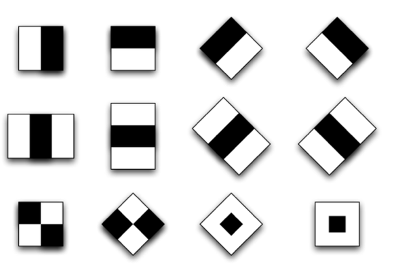
\includegraphics[scale=1]{image2-4}
%  \caption{نمونه هایی از مستطیل های ویژگی های Haar \cite{990517}.}
%  \label{image2-4}
%\end{figure}
%
%\noindent
%ویژگی‌های‌ \lr{Haar} برای تشخیص چشم، بینی، دهان و... با کمک تشخیص لبه، تشخیص خط و تشخیص مرکز در تصویر و استخراج ویژگی برای یافتن چهره استفاده می‌شود. مستطیل‌های ویژگی‌های \lr{Haar}، متناسب با بخش‌های چهره می‌باشند که مثالی از آن در شکل \ref{image2-5} نشان داده شده است.
%
%\begin{figure}
%	\centering
%	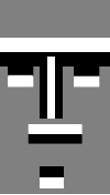
\includegraphics[scale=1]{image2-5}
%	\caption{مستطیل های ویژگی های Haar متناسب با بخش های چهره می باشند \cite{990517}.}
%	\label{image2-5}
%\end{figure}
%
%\noindent
%همانطور که در شکل \ref{image2-6} مشاهده می‌شود، هر مستطیل در بخش‌های مختلف چهره در روندی تکراری با اندازه‌های مختلف قرار می‌گیرد و نتیجه نهایی از کم کردن مجموع سطح روشنایی پیکسل‌های زیر بخش‌های سیاه از مجموع سطح روشنایی پیکسل‌های زیر بخش‌های سفید به دست می‌آید که یک عدد می‌باشد. از یک پنجره با اندازه ۲۴×۲۴ برای قرار دادن مستطیل‌ها بر روی تصویر استفاده می‌شود که تعداد زیاد و اندازه‌های مختلف آن‌ها باعث می‌شود برای محاسبه نتیجه نهایی نیاز به انجام بیش از ۱۶۰۰۰۰ محاسبه باشد که زمان زیادی برای هر تصویر خواهد گرفت.
%
%\begin{figure}[h]
%\centering
%  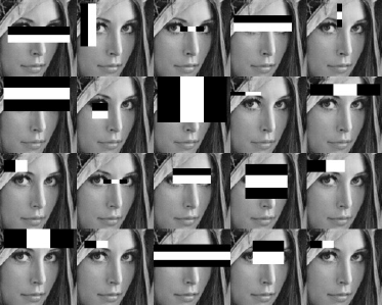
\includegraphics[scale=1]{image2-6}
%  \caption{هر مستطیل در اندازه های مختلف بر روی بخش های مختلف تصویر قرار می گیرد \cite{990517}.}
%  \label{image2-6}
%\end{figure}
%
%\noindent
%\lr{Ada Boost}: 
%تمام ویژگی‌های Haar برای تصویر ورودی مناسب نخواهد بود. بعضی از این ویژگی‌ها باید نادیده گرفته شوند و فقط ویژگی‌های مرتبط انتخاب شوند تا در زمان صرفه جویی شود. این کار به صورت خودکار به کمک عنصر \lr{Ada Boost} انجام می‌شود. \lr{Ada Boost} یک الگوریتم مبتنی بر یادگیری ماشین می‌باشد که ویژگی‌های کاربردی را از میان تعداد زیادی ویژگی پیدا می‌کند. بعد از شناسایی ویژگی‌های مختلف، مشخص می‌گردد که هر یک از پنجره‌ها برای بخشی از چهره مناسب می‌باشد یا خیر. هر کدام از ضرایب انتخاب شده مثبت در نظر گرفته می‌شود، در صورتی که حداقل بتواند بیش از نیمی از موارد را تشخیص دهد. این ویژگی‌ها با عنوان طبقه‌بندهای ضعیف \LTRfootnote{Weak Classifier} معرفی می‌شوند. \lr{Ada Boost}  در طبقه‌بند قوی \LTRfootnote{Strong Classifier}، تعداد زیادی طبقه‌بند ضعیف را با هم ترکیب می‌کند. رابطه کلی آن به صورت زیر می‌باشد.
%
%\begin{equation}\label{eq2-5}
%F(x)=\alpha_1 f_1 (x) + \alpha_2 f_2 (x) + \cdots
%\end{equation}
%
%\noindent
%که در آن \lr{F} طبقه‌بند قوی می‌باشد که از تعدادی $f_i$ که طبقه‌بند ضعیف می‌باشد، تشکیل شده است. هر کدام از طبقه‌بندهای ضعیف، یک خروجی صفر یا یک تولید می‌کنند. $\alpha_i$ وزن مربوط به طبقه‌بند می‌باشد. با استفاده از این الگوریتم و وزن دادن به ویژگی‌ها، بیش از ۱۶۰۰۰۰ ویژگی قبلی به کمتر از ۲۵۰۰ ویژگی کاهش پیدا می‌کند.
%
%\noindent
%مراحل آبشاری \LTRfootnote{Cascading}: اگر تصویر به مربع‌های ۲۴×۲۴ پیکسلی تقسیم شده و با پردازش هر بخش که ۲۵۰۰ ویژگی دارد، تشخیص داده شود که چهره‌ای در تصویر وجود دارد یا خیر، حجم محاسبات بسیار زیاد خواهد بود. مراحل آبشاری این فرایند را سریع‌تر انجام می‌دهد. ۲۵۰۰ ویژگی هر مربع ۲۴×۲۴ به دسته‌بندی‌های مختلف تقسیم می‌شود. برای مثال ۱۰ ویژگی در دسته‌ اول، ۲۰ ویژگی در دسته دوم، ۱۰۰ ویژگی در دسته سوم و... . می‌توان بعد از پردازش هر دسته، در ارتباط با وجود یا عدم وجود چهره در آن دسته تصمیم گرفت تا بخش‌هایی که چهره در آن وجود ندارد زودتر حذف شوند. شکل \ref{image2-10} یک نمای کلی از روند تشخیص آبشاری را نشان می‌دهد. مجموعه ای از طبقه‌بندها به هر زیر پنجره اعمال می‌شود. طبقه بند اولیه تعداد زیادی از نمونه‌های منفی را حذف می‌کند و پردازش کمی دارد. لایه‌های بعد، منفی‌های اضافی را حذف می‌کنند که نیاز به محاسبات بیشتری دارند. این الگوریتم عملکرد بسیار خوبی در برنامه‌های کاربردی بی‌درنگ و در حضور پس زمینه‌های شلوغ نشان داده است. اما هنوز در برای چهره‌هایی که رو به روی دوربین نیستند، تغییرات شدید نور، انسداد و... دارای چالش می‌باشد.
%
%\begin{figure}[h]
%\centering
%  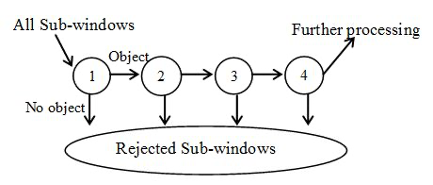
\includegraphics[scale=1]{image2-10}
%  \caption{بخشی از یک تصویر که مراحل آبشاری برای آن محاسبه می‌شود \cite{990517}.}
%  \label{image2-10}
%\end{figure}

\noindent
در سال ۲۰۰۵ \lr{Dalal} و همکاران \cite{1467360} روشی به نام بافت نگار شیب‌های جهت دار \LTRfootnote{Histograms Of Oriented Gradients} ارائه کردند که به اختصار \lr{HOG} نامیده می‌شود. در این روش ابتدا تصویر خاکستری می‌شود، زیرا نیازی به رنگ نیست. پیرامون هر پیکسل بررسی می‌شود تا مشخص شود نسبت به پیکسل‌های پیرامونش چقدر تاریک می‌باشد. مطابق شکل \ref{image2-11} جهتی انتخاب می‌شود که به سمت پیکسل‌های تاریکتر باشد. این روند برای همه پیکسل‌های تصویر انجام می‌شود و به ازای هر پیکسل یک جهت ذخیره خواهد شد که روندی از روشنایى به تاریكى را در تصویر نمایش می‌دهند.

\begin{figure}
	\centering
	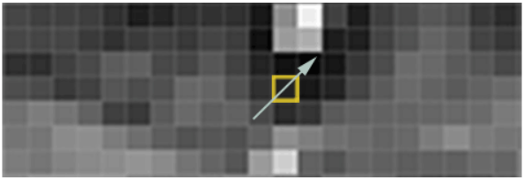
\includegraphics[scale=0.5]{image2-11}
	\caption{سطح روشنایی پیکسل های اطراف هر پیکسل بررسی شده و راستای روشن به سمت تاریک برگزیده می شود \cite{1467360}.}
	\label{image2-11}
\end{figure}

\noindent
دلیل استفاده از جهت‌ها این است که اگر پیکسل‌ها به طور مستقیم استفاده شوند، تصویر تاریك و تصویر روشن از یك چهره مشخص، دارای سطح روشنایی متفاوتى خواهند بود. اما با در نظر گرفتن جهتى تغییر روشنایى، هم تصویر تیره و هم تصویر روشن، نمایش یكسانى خواهند داشت كه حل مسئله را آسان‌تر می‌كند. ذخیره جهت‌ها براى تمام پیکسل‌ها باعث افزایش جزئیات می‌شود. لذا روند اصلى روشنایى و تاریكى در سطحی بالاتر در نظر گرفته می‌شود، به طورى كه بتوان الگوى اصلى تصویر را دید. تصویر به بخش‌هاى ١٦×١٦ پیكسل تقسیم می-شود و در هر بخش تعداد جهت‌هاى به سمت بالا، پایین، چپ و راست شمارش می‌شود. سپس بخش‌هاى درون تصویر با جهت‌هایى كه بزرگتر بودند، جایگزین می‌شود. نتیجه نهایى، تبدیل تصویر به یك نمایش ساده شده از ساختار چهره است که در شکل \ref{image2-12} مشاهده می‌شود. براى یافتن چهره‌ها در این الگوریتم، بخش‌هایى از تصویر كه به الگوى \lr{HOG} شبیه‌تر است، مشخص می‌شود. با استفاده از این روش، می‌توان چهره‌ها را در تصویر به سادگى پیدا كرد.

\begin{figure}
	\centering
	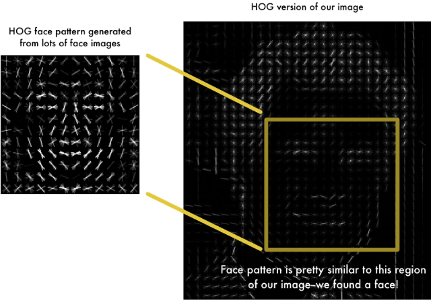
\includegraphics[scale=1]{image2-12}
	\caption{براى یافتن چهره ها، بخش هایى از تصویر كه به الگوى HOG شبیه تر است را پیدا می كنیم \cite{1467360}.}
	\label{image2-12}
\end{figure}

\noindent
در سال 2015 \lr{Shengcai Liao} و همکاران \cite{7130626} یک روش دقیق و سریع برای یافتن چهره ارائه دادند که در آن از اختلاف پیکسل هنجارسازی شده یا \lr{NDP} \LTRfootnote{Normalized Pixel Difference} برای یافتن چهره استفاده می‌شود. ارزیابی ویژگی \lr{NPD} بسیار سریع است و دسترسی به حافظه تنها با استفاده از یک جدول جستجو می‌باشد. در این روش نشانه گذاری یا خوشه بندی در مرحله آموزش نیز لازم نیست و در برابر تغییرات نور، حالت، انسداد، تصاویر با وضوح پایین و... مقاوم است. \lr{NPD} بین دو پیکسل در یک تصویر به صورت زیر تعریف شده است:
\begin{equation}\label{eq2-6}
f(x, y) = \frac{x - y}{x + y}
\end{equation}

\noindent
که در آن $x$ و $y$ بزرگتر از صفر هستند و $f(0,0)$ برای حالتی که $x = y = 0$ باشد، برابر صفر است. این عمل بر روی هر جفت پیکسل از تصویر اجرا می‌شود. اگر تصویر ورودی مربعی با ابعاد $s$ باشد و $p=s \times s$ تعداد پیکسل‌ها باشد، آنگاه تعداد ویژگی‌های استخراج شده برابر $d=p(p-1)/2$ می‌باشد. سپس علامت \LTRfootnote{Sign} ویژگی‌های استخراج شده مورد استفاده قرار می‌گیرد که وابسته به اندازه سطح روشنایی پیکسل‌ها نمی‌باشد. بلکه تنها نشان می‌دهد کدام ناحیه روشن‌تر و کدام ناحیه تیره‌تر می‌باشد. همچنین این ویژگی‌ها به خدشه \LTRfootnote{Noise} حساس نمی‌باشند. در نهایت ویژگی‌های استخراج شده به عنوان ورودی به یک سامانه یادگیری داده می‌شود. نمونه‌ای از نتیجه اجرای این الگوریتم بر روی مجموعه داده \lr{FDDB} در شکل \ref{image2-13} آمده است.
 
 \begin{figure}[h]
\centering
  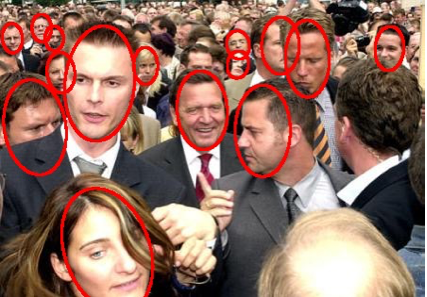
\includegraphics[scale=1]{image2-13}
  \caption{نتیجه اجرای روش مبتنی بر NPD \cite{7130626}.}
  \label{image2-13}
\end{figure}

\noindent
تمام رویکرد‌های ارائه شده که یافتن چهره را با مدل سازی صریح از ویژگی‌های صورت انجام می‌دهند، در برابر تغییرات غیر قابل پیش بینی چهره و شرایط محیطی دچار مشکل می‌شوند. اگرچه بعضی از تلاش‌های اخیر مبتنی بر ویژگی، توانایی مقابله با شرایط کنترل نشده را بهبود داده‌اند، اما بیشتر آن‌ها هنوز به چهره‌های رو به رو و شرایط کنترل شده محدود می‌شوند، و به عنوان یکی از روش‌های یک سامانه ترکیبی در نظر گرفته شده‌اند. پس نیاز به روش‌هایی هست که بتوانند در شرایط خصمانه تر مانند تشخیص چهره‌های متعدد در زمینه‌های شلوغ به خوبی عمل کنند.

 \subsection{رویکردهای مبتنی بر یادگیری}
با توجه به آنچه در \cite{8253595} آمده است، چالش اصلی در یافتن چهره این است که ویژگی‌هایی مانند \lr{Haar} و \lr{HOG} اطلاعات برجسته چهره را در شرایط مختلف نما، نورپردازی، رنگ پوست، انسداد، استفاده از لوازم آرایشی و... استخراج نمی‌کنند. این محدودیت بیشتر به دلیل ویژگی‌های استفاده شده در طبقه‌بندها است. با پیشرفت‌های اخیر در رویکردهای یادگیری عمیق و در دسترس بودن پردازنده‌های گرافیکی، استفاده از شبکه‌های عصبی پیچشی عمیق برای استخراج ویژگی امکان پذیر شده است. 

\noindent
در سال ۲۰۱۹ \lr{Deng} و همکاران \cite{deng2019retinaface} یک روش مبتنی بر شبکه عصبی پیچشی برای یافتن چهره در تصویر پیشنهاد کردند.‌ در این روش برای آموزش شبکه پیچشی از یک تابع ضرر مبتنی بر یادگیری چندکاره \LTRfootnote{Multi Task Learning} استفاده شده است که به صورت رابطه \ref{eq2-7} می‌باشد.
\begin{equation}\label{eq2-7}
L = L_{cls} + L_{box} + L_{pts} + L_{pixel}  
\end{equation}

\noindent
که در آن $L_{cls}$ تابع ضرر مربوط به یافتن یا عدم یافتن چهره می‌باشد. $L_{box}$ تابع ضرر مربوط به مکان چهره می‌باشد. همچنین $L_{pts}$ تابع ضرر مربوط به یافتن نقاط ویژه روی اجزای چهره می‌باشد، و $L_{pixel}$ تابع ضرر مربوط به یافتن یک مدل سه بعدی مبتنی بر مش از روی چهره می‌باشد. استفاده از تابع ضرر مبتنی بر یادگیری چند کاره، کمک می نماید تا فضای مسئله محدود تر شود و الگوریتم بهینه سازی مورد نظر زودتر به سمت نقطه بهینه همگرا شود. شمای کلی این روش را در شکل \ref{image2-14} مشاهده می‌کنید. 

\begin{figure}[h]
\centering
  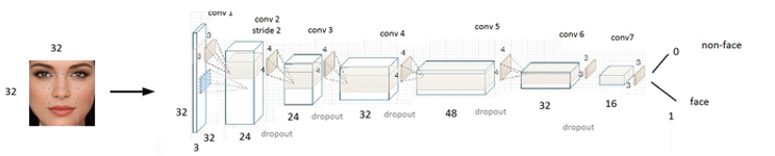
\includegraphics[width=1.0\textwidth]{image2-14}
  \caption{
نمای کلی روش یافتن چهره تک مرحله ای و متراکم.  \lr{RetinaFace} بر اساس هرم ویژگی طراحی شده است. این رویکرد از تابع ضرر چند کاره استفاده می‌نماید.
 \cite{deng2019retinaface}.}
  \label{image2-14}
\end{figure}

\noindent
نمونه ای از خروجی این روش را در شکل \ref{image2-15} مشاهده می‌کنید. 
\begin{figure}[h]
	\centering
	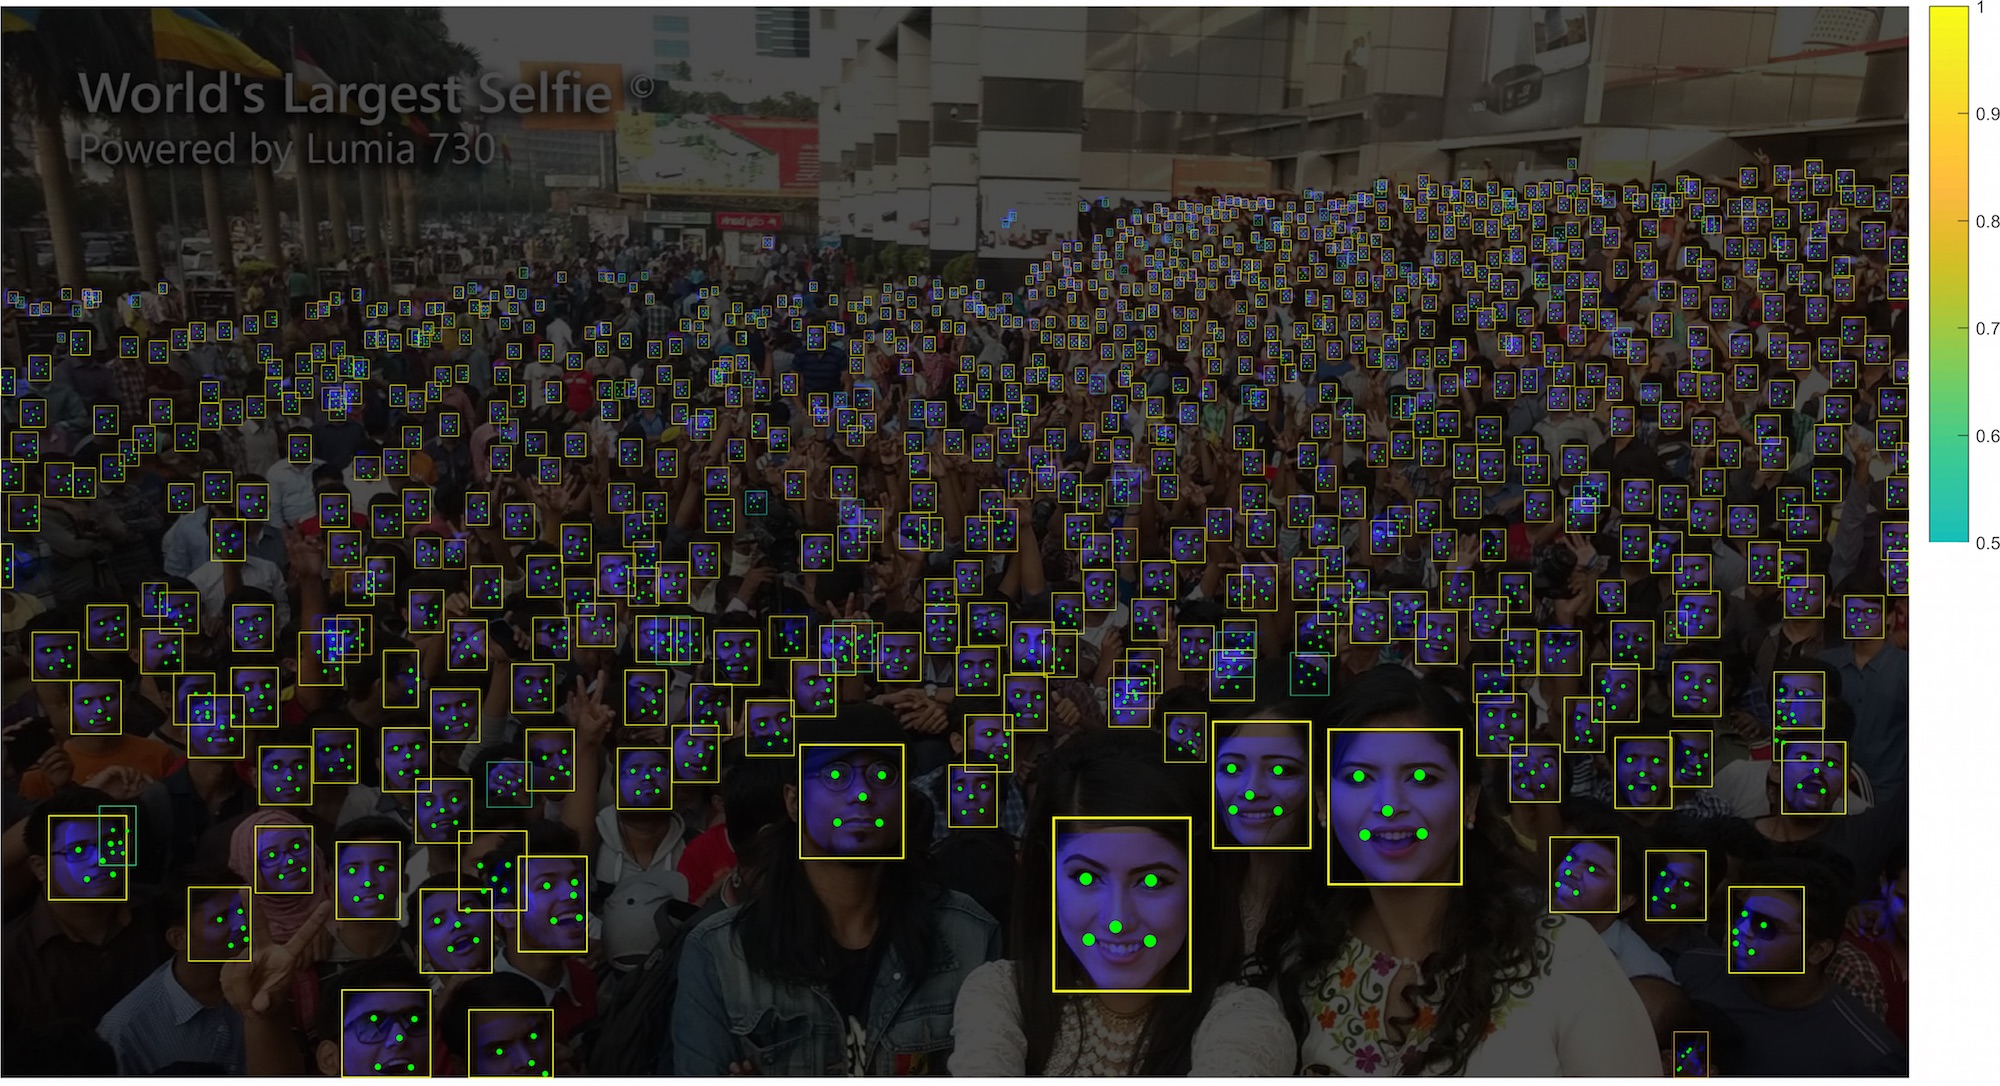
\includegraphics[width=1.0\textwidth]{image2-15}
	\caption{نمونه از خروجی الگوریتم یافتن چهره retina \cite{deng2019retinaface}.}
	\label{image2-15}
\end{figure}

\section{شناسایی چهره}
شناسایی چهره در دو مرحله انجام می‌شود. مرحله اول استخراج ویژگی و مرحله دوم، طبقه‌بندی است. الگوریتم‌های شناسایی چهره را می‌توان به دو دسته اصلی تقسیم کرد. الگوریتم‌های هندسی که بر مبنای استخراج ویژگی‌های متمایز چهره‌ها کار می‌کنند، و الگوریتم‌های تصویری که تصویر را تبدیل به یک الگو می‌نماید و الگوها را مقایسه می‌نماید. رویکردهای مختلفی برای شناسایی چهره طراحی شده است که در ادامه مهم‌ترین آن‌ها آمده است.

\subsection{رویکرد‌های سنتی}
این رویکردها ویژگی‌های چهره را با علامت‌ها و اندازه‌ها از تصویر استخراج می‌کنند. برای مثال موقعیت نسبی، اندازه و یا شکل چشم‌ها، بینی، گونه‌‌ها و فک را محاسبه کرده و تجزیه و تحلیل می‌کنند. سپس از این ویژگی‌ها برای جستجوی تصاویر دیگر در پایگاه داده استفاده می‌کنند. در سال 1993 \lr{Roberto Brunelli} و همکاران \cite{254061} یکی از اولین الگوریتم‌ها در این زمینه را ارائه دادند که رویکرد‌ موفقی مبتنی بر روش‌های تطبیق الگو داشت. این رویکرد در شرایط کنترل شده به دقت 90\% رسید.
 
\subsection{رویکرد مبتنی بر فیلتر گابور ‌}
در سال ۲۰۰۷ \lr{A. F. Abate} و همکاران \cite{ABATE20071885} یک رویکرد مبتنی بر فیلتر گابور ارائه دادند. در این رویکرد ابتدا تصویر را بخش بندی \LTRfootnote{Grid} کرده، سپس بر روی بخش‌های مختلف آن، فیلتر گابور \LTRfootnote{Gabor} اعمال می‌شود و نتیجه بدست آمده با یک طرح از پیش آماده شده، با یک آستانه گذاری مطابقت داده می‌شود. شکل \ref{image2-17} فیلترهای چندگانه گابور و تاثیر این فیلترها بر روی تصویر چهره انسان را نشان می‌دهد. دلیل استفاده از فیلتر گابور این است که عملکرد این فیلتر به سامانه بصری انسان بسیار شباهت دارد. 
 	 
\begin{figure}
\begin{subfigure}{.5\textwidth}
  \centering
  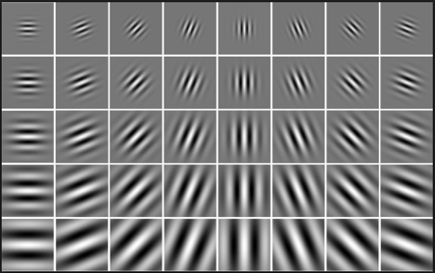
\includegraphics[width=1.0\textwidth]{image2-17-a}
  \caption{ }
  \label{image2-17-a}
\end{subfigure}
\begin{subfigure}{.5\textwidth}
  \centering
  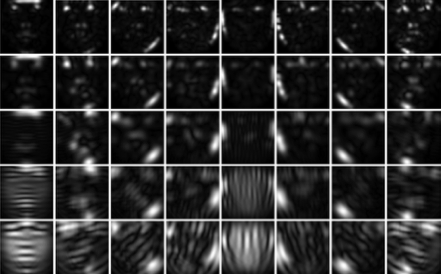
\includegraphics[width=1.0\textwidth]{image2-17-b}
  \caption{ }
  \label{image2-17-b}
\end{subfigure}
  \caption{(آ) فیلترهای چندگانه گابور (ب) تاثیر این فیلترها بر روی تصویر چهره \cite{ABATE20071885}.}
\label{image2-17}
\end{figure}

\subsection{رویکرد‌های سه بعدی}
در سال ۲۰۰۹ \lr{JafriRabia} و همکاران \cite{10.3745/JIPS.2009.5.2.041} نشان داده‌اند که داده‌های سه بعدی دقت تشخیص چهره را به شدت بهبود می‌بخشد. روش تشخیص سه بعدی چهره از یک منتشر کننده نور فرو سرخ و یک حسگر به عنوان دریافت کننده استفاده می‌کند. شبکه‌ای از نورهای فرو سرخ که برای انسان قابل رویت نیست، روی چهره تابانده می‌شود. سپس یک حسگر ویژه، پرتوهای بازتاب را دریافت کرده و اطلاعات عمق تصویر پردازش می‌شود. این دسته از الگوریتم‌ها برای شناسایی دقیق اشخاص، برای هر نفر برداری‌های سه بعدی می‌سازند. عیب رویکردهای سه بعدی، نیاز به تجهیزات پیشرفته و غیر قابل استفاده بودن در شرایط کنترل نشده مانند خیابان و معابر پیاده می‌باشد. شکل \ref{image2-18} یک مدل سازی سه بعدی چهره با اشعه فروسرخ را نشان می‌دهد.

\begin{figure}[h]
\centering
  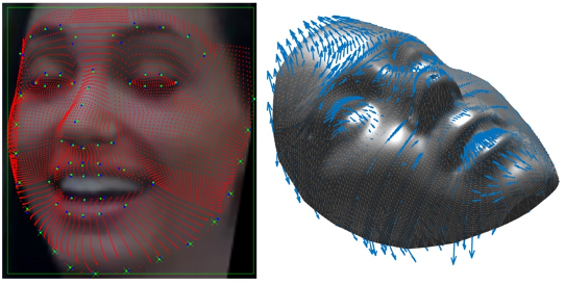
\includegraphics[scale=1]{image2-18}
  \caption{مدل سازی سه بعدی چهره با اشعه فرو سرخ \cite{10.3745/JIPS.2009.5.2.041}.}
  \label{image2-18}
\end{figure}

\noindent
در سال 2017 \lr{Guosheng Hu} و همکاران \cite{HU2017366} یک روش سه بعدی برای توصیف ویژگی‌های چهره ارائه کردند که در آن از مدل سازی سه بعدی چهره به همراه تجزیه و تحلیل بافت پوست استفاده شده است. یکی دیگر از رویکردهای در حال ظهور، استفاده از بافت پوست برای شناسایی چهره می‌باشد که خطوط، الگوها و لکه‌های پوست را به یک فضای ریاضی تبدیل می‌کند. تجزیه و تحلیل بافت بسیار شبیه روش شناسایی چهره است. تصویری از پوست گرفته می‌شود و به بخش‌های کوچکتر تقسیم می‌شود. سپس هر بخش به یک فضای ریاضی قابل اندازه گیری تبدیل می‌شود و خطوط، منافذ و بافت پوست تشخیص داده می‌شود. این رویکرد می‌تواند تفاوت بین دوقلوهای یکسان را شناسایی کند که با استفاده از تشخیص چهره به تنهایی امکان پذیر نیست. آزمایش‌ها نشان دادند که با افزودن تحلیل بافت پوست، عملکرد سامانه تشخیص چهره می‌تواند 20 تا 25 درصد افزایش یابد. این سامانه شایستگی استفاده در کاربردهای مختلف امنیتی و نظامی با شناسایی خودکار سریع و بدون دخالت شخص را دارد و سرعت پردازش را بالا و خطا را کاهش داده است. برتری روش سه بعدی در عدم وابستگی به حرکت و جا به جایی صورت است. انتقال و نصب سامانه تصویر برداری بسیار ساده است. زاویه دید حسگر چندان مهم نیست. همچنین نورپردازی نامناسب تاثیری در این شیوه ندارد و عملیات آن ساده است. بر خلاف روش تشخیص دو بعدی، روش سه بعدی و تجزیه و تحلیل بافت پوست به تجهیزات بسیار پیچیده تری نیاز دارد، و با توجه به آنکه تمرکز ما بر روی تشخیص چهره به صورت بی‌درنگ در شرایط کنترل نشده مانند معابر پیاده و خیابان می‌باشد، به توضیح مختصر رویکردهای سه بعدی و تجزیه و تحلیل بافت پوست بسنده می‌کنیم.

\subsection{رویکرد‌های مبتنی بر دوربین حرارتی}
در این رویکرد، دوربین حرارتی شکل صورت را تشخیص می‌دهد و از لوازم جانبی مانند عینک، کلاه یا آرایش چشم پوشی می‌کند. بر خلاف دوربین‌های معمولی، دوربین‌های حرارتی می‌توانند تصاویر را حتی در شرایط کم نور مانند شب، بدون استفاده از فلاش و قرار گرفتن در معرض مستقیم دوربین ضبط کنند. با این حال، یکی از مشکل‌های استفاده از تصاویر حرارتی برای تشخیص چهره این است که مجموعه داده‌های آن برای شناسایی چهره محدود است.

\noindent
در سال 2003 \lr{Diego Socolinsky} و همکاران \cite{SOCOLINSKY200372} از شناسایی چهره مبتنی بر دوربین حرارتی در کاربردهای واقعی بهره برداری کردند و یک مجموعه داده جدید از تصاویر حرارتی چهره ایجاد کردند. آن‌ها از حسگرهای الکتریکی فروسرخ با حساسیت کم و با توانایی جذب حرارت طولانی مدت یا \lr{LWIR} \LTRfootnote{Longwave Infrared} استفاده کردند. نتایج نشان می‌دهد که تلفیق \lr{LWIR} و دوربین‌های معمولی، نتایج بهتری در شرایط کنترل نشده دارد. در این مطالعه 240 چهره مجزا در طی 10 هفته برای ایجاد پایگاه داده جدید استفاده شده است. داده‌ها در روزهای آفتابی، بارانی و ابری جمع آوری شد. در شرایط کنترل شده دوربین معمولی دقت ۹۷٫۰۵٪ درصد دارد، در حالی که روش \lr{LWIR} دارای دقت ۹۳٫۹۳٪ می‌باشد و ترکیب این دو دارای دقت ۹۸٫۴۰٪ است. در شرایط کنترل نشده دوربین معمولی دقت ۶۷٫۰۶٪، دوربین \lr{LWIR} دقت ۸۳٫۰۳٪ و ترکیب این دو دارای دقت ۸۹٫۰۲٪ است.

\subsection{تشخیص چهره مبتنی بر ویدیو}
در سال 2009 \lr{Huafeng Wang} و همکاران \cite{wang2009video} یک برآورد کلی از رویکردهای مبتنی بر ویدیو ارائه دادند. تشخیص چهره در ویدیو در طی چند سال گذشته مورد توجه قرار گرفته و طیف گسترده‌ای از برنامه‌های کاربردی تجاری و اجرای قانون را در بر گرفته است. فیلم‌ها قادر به ارائه اطلاعات بیشتر نسبت به تصاویر ثابت هستند. مزایای عمده استفاده از ویدیو عبارتند از:

\begin{enumerate}
\item
	امکان استفاده از افزونگی موجود در توالی ویدیو برای بهبود عملکرد تشخیص نسبت به تصاویر ثابت وجود دارد. تشخیص چهره و پیگیری آن در طول زمان، موجب انتخاب فریم‌های خوب می‌شود که حاوی چهره‌های رو به رو یا نشانه‌های ارزشمند است که شرایط نور، انسداد، حالت چهره و... در آن رضایت بخش می‌باشد.

\item
	نمایش‌های موثرتر مانند مدل چهره سه بعدی یا تصاویر \lr{super resolution} می‌توانند از اطلاعات فریم‌های ویدیو گرفته شده برای بهبود شناخت استفاده کنند.

\item
	یادگیری و به روز رسانی مدل در طول زمان امکان پذیر می‌باشد.
\end{enumerate}
	
\noindent
برای تشخیص چهره در تصاویر ویدیویی، دو رویکرد کلی وجود دارد:

\noindent
مبتنی بر قاب \LTRfootnote{Frame}: در این رویکرد برای شناسایی چهره، هر قاب به صورت جداگانه مورد پردازش قرار می‌گیرد که عیب آن نادیده گرفتن اطلاعات زمانی ارائه شده توسط توالی ویدیویی می‌باشد. 

\noindent
یافتن و ردیابی \LTRfootnote{Detection And Tracking}: یافتن چهره در اولین قاب و سپس ردیابی آن از طریق توالی قاب‌ها. شکل \ref{image2-19} نمای کلی این رویکرد را نشان می‌دهد.
 
 \begin{figure}[h]
\centering
  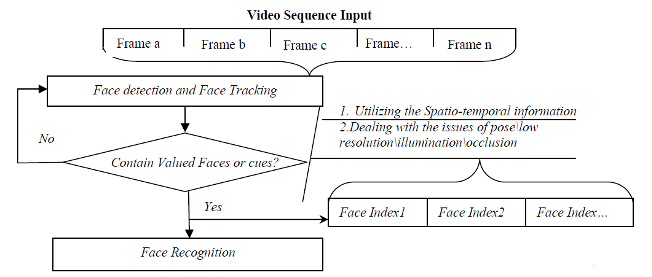
\includegraphics[width=1.0\textwidth]{image2-19}
  \caption{نمای کلی یک سامانه تشخیص چهره مبتنی بر یافتن چهره و ردیابی آن \cite{wang2009video}.}
  \label{image2-19}
\end{figure}

 \subsection{رویکرد مبتنی بر چهره ویژه}
با افزایش حجم داده‌های موجود، نیاز به کاهش ابعاد داده‌ها می‌باشد. تحلیل مؤلفه‌های اساسی یا \lr{PCA} \LTRfootnote{Principle Component Analysis} یک روش‌ کاهش ابعاد داده‌ها است که در برخی مسئله‌ها مانند پردازش تصویر به خوبی و با سرعت بالا عمل می‌کند. استفاده از این روش در پردازش سریع‌تر داده‌ها کمک می‌کند و از رخ دادن مشکل ‌بیش‌برازش \LTRfootnote{Overfiting} جلوگیری می‌نماید. اگر یک پایگاه داده عظیم از تصاویر چهره اشخاص با وضوح بالا موجود باشد که هر کدام دارای تعدادی زیاد ویژگی هستند، و بخواهیم یک تصویر آزمایش را با این پایگاه داده مقایسه کرده و شخص شبیه به آن را پیدا کنیم، مقایسه تصاویر بسیار زمان بر و در مواردی غیر ممکن خواهد بود. \lr{PCA} در این مسئله به خوبی عمل می‌کند. با اعمال تکنیک کاهش بعد به تصویر و با به دست آوردن تصویر ویژه چهره‌ها \LTRfootnote{Eigenface} می‌توان ویژگی‌ها را کاهش داد و نتیجه مطلوب را در زمان بسیار کم گرفت. شکل \ref{image2-20} تعدادی چهره و چهره‌های ویژه متناظر با آن‌ها را نشان می‌دهد.

\noindent
در سال 2014 \lr{Xiao Luan} و همکاران \cite{LUAN2014495} یک روش تشخیص چهره مبتنی بر \lr{PCA} ارائه دادند که تا حدی در برابر تغییرات نورپردازی و انسداد مقاوم می‌باشد. \lr{PCA} راستای بیشترین تغییرات را با توجه به تعداد ویژگی‌ها و نوع آن‌ها به ما می‌دهد. به همین دلیل در برخی موارد که تنها محوری که بیشترین تغییرات یا پراکندگی را دارد برای ما مهم است، راه حل مناسبی خواهد بود. 

\begin{figure}
\begin{subfigure}{.5\textwidth}
  \centering
  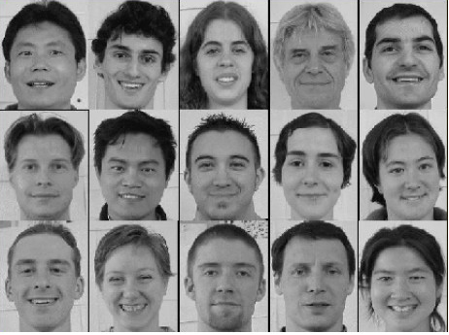
\includegraphics[width=1.0\textwidth]{image2-20-a}
  \caption{ }
  \label{image2-20-a}
\end{subfigure}
\begin{subfigure}{.5\textwidth}
  \centering
  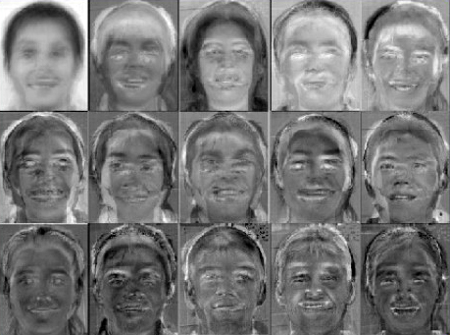
\includegraphics[width=1.0\textwidth]{image2-20-b}
  \caption{ }
  \label{image2-20-b}
\end{subfigure}
  \caption{ (آ) تعدادی چهره و (ب) چهره های ویژه متناظر با آن ها \cite{LUAN2014495}.}
\label{image2-20}
\end{figure}

\noindent
در سال 2016 \lr{K. R. Sreelakshmi} و همکاران \cite{7854053} یک روش شناسایی چهره مبتنی بر چهره‌های ویژه ارائه دادند که در آن ابتدا تصویر ورودی با استفاده از ماتریس بردارهای ویژه، به فضای دیگری منتقل می‎شود، سپس در فضای کاهش بعد یافته با داده‌های موجود مقایسه شده و شبیه‌ترین تصویر به آن انتخاب می‌شود. برای مقایسه از معیارهایی مانند معیار اقلیدسی و منهتن می‌توان استفاده کرد. از مزایای این روش می‌توان به سهولت پیاده‌سازی و استفاده، کاهش حجم داده‌ها و سرعت بالا اشاره کرد. در نظر نگرفتن پراکندگی درون کلاسی و بین کلاسی داده‌ها، عدم توجه به برچسب تصویر برای شناسایی، تمایز قایل نشدن بین تصاویر مختلف یک شخص در پایگاه و نیاز به بروز رسانی تمامی اطلاعات موجود با ورود یک تصویر جدید به پایگاه داده از معایب این روش است. 
محاسبات ریاضی و مراحل انجام آن‌ها:
\begin{enumerate}
\item
	تبدیل ماتریس تصاویر به بردار و کنار هم قرار دادن آن‌ها برای تشکیل ماتریس داده‌ها
\item 
	محاسبه‏ میانگین ماتریس بدست آمده و انتقال داده‌ها به مرکزیت صفر
\item
	محاسبه‏ ماتریس کوواریانس بردارها و مقادیر ویژه‏ آن
\item
	انتقال ماتریس داده‌ها به زیرفضای جدید با استفاده از ماتریس بردارهای ویژه
\item
	بررسی شباهت بین بردار منتقل شده و بردارهای موجود و انتخاب شبیه‌ترین بردار
\end{enumerate}
 
\subsection{رویکردهای مبتنی بر یادگیری عمیق}
یک راه حل غیر خطی برای شناسایی چهره، استفاده از شبکه‌ عصبی پیچشی است که به طور شگفت انگیزی در طبقه‌بندی تصاویر چهره خوب کار می‌کند و ویژگی‌های ارزشمندی را از تصویر چهره استخراج می‌کند. بنابراین می‌توان از آن در حل مسئله شناسایی چهره‌ و تأیید هویت استفاده کرد. شکل \ref{image2-21} ساختار کلی یک شبکه عصبی عمیق برای شناسایی چهره را نشان می‌دهد.
 
\begin{figure}[h]
\centering
  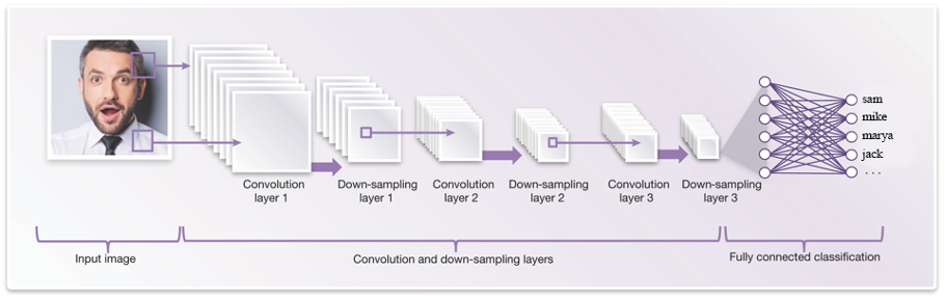
\includegraphics[width=1.0\textwidth]{image2-21}
  \caption{شبکه عصبی عمیق برای شناسایی چهره \cite{cnn}.}
  \label{image2-21}
\end{figure}

\noindent
معمولا به عنوان تابع فعالیت از توابع غیرخطی مانند \lr{ReLU} \LTRfootnote{Rectified Linear Unit} استفاده می‌شود. و عملیات بهینه سازی به روش پس انتشار خطا انجام می گردد. و در لایه خروجی از تابع \lr{SoftMax} برای طبقه‌بندی استفاده می‌شود که خروجی های لایه آخر را هنجار می‌کند. شبکه‌های عصبی پیچشی ویژگی‌های یک چهره را استخراج می‌کنند که می‌توان به عنوان یک شناسه برای یک فرد خاص در نظر گرفت. هنگامی که دو تصویر مختلف از چهره یک شخص به عنوان ورودی داده می‌شود، شبکه باید خروجی‌های مشابه (ویژگی‌های نزدیک تر) را برای هر دو تصویر تولید نماید، در حالی که برای چهره دو شخص مختلف، شبکه باید خروجی‌های بسیار متفاوت برای دو تصویر تولید نماید. شبکه عصبی نیاز به آموزش دارد تا به طور خودکار ویژگی‌های مختلف چهره‌ها را شناسایی کند و بر اساس آن محاسبات را انجام دهد. در ادامه چند شبکه عصبی پیچشی معروف مورد بررسی قرار گرفته است.

\subsubsection{	شبکه \lr{FaceNet}}
در سال 2015 \lr{Florian Schroff} و همکاران \cite{7298682} یک شبکه عصبی عمیق به نام \lr{FaceNet} ارائه دادند. \lr{FaceNet} یک مدل یکپارچه است که می‌آموزد چگونه تصاویر چهره را به یک فضای اقلیدسی فشرده نگاشت دهد تا فاصله تصاویر به طور مستقیم با میزان شباهت چهره‌ها مرتبط باشد. هنگامی که این فضا تولید شود، شناسایی چهره، تایید هویت و خوشه‌بندی می‌تواند به راحتی با استفاده از روش‌های استاندارد توسط \lr{FaceNet} انجام شود. این شبکه برای آموزش از سه گانه تطبیق – عدم تطبیق استفاده می‌نماید. با توجه به شکل \ref{image2-22}، سه گانه تطبیق – عدم تطبیق یک مجموعه از سه تصویر شامل یک تصویر لنگر\LTRfootnote{Anchor}، یک تصویر منطبق بر تصویر لنگر (مثبت\LTRfootnote{Positive}) و یک تصویر غیر منطبق بر تصویر لنگر (منفی\LTRfootnote{Negative}) است که باید فاصله بین تصویر لنگر و تصویر مثبت را به حداقل برساند، زیرا هر دو دارای هویت مشابه هستند و فاصله بین تصویر لنگر و تصویر منفی را به حداکثر برساند، زیرا این تصاویر دارای هویت متفاوت می‌باشند. 
 
\begin{figure}[h]
\centering
  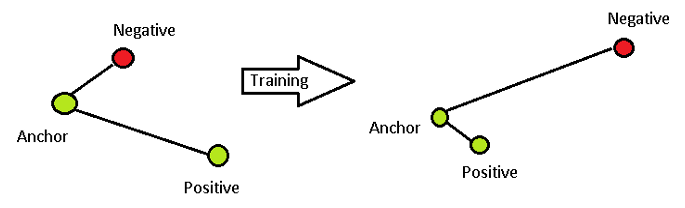
\includegraphics[width=0.5\textwidth]{image2-22}
  \caption{سه گانه تطبیق – عدم تطبیق \cite{7298682}.}
  \label{image2-22}
\end{figure}

\noindent 
برای هر داده آموزشی \lr{A} مجموعه‌ای از داده‌های مثبت و مجموعه‌ای از داده‌های منفی در نظر گرفته می‌شود. سپس داده‌ها با تابع ضرر سه گانه طوری آموزش می‌بینند که رابطه \ref{eq2-10} برای هر کدام از داده‌های آموزشی برقرار باشد.
\begin{equation}
\label{eq2-10}
‖f(A)-f(P)‖^2≤‖f(A)-f(N)‖^2	
\end{equation}

\noindent
که در آن تابع $f$ ویژگی‌های استخراج شده از تصاویر است. شبكه در مرحله آموزش با استفاده از داده‌های برچسب‌گذاری شده، می‌آموزد فاصله بین ویژگی‌های شبیه به هم، کمتر از فاصله بین ویژگی‌های دور باشد و به این ترتیب در مرحله آزمایش می‌تواند داده‌های مثبت و منفی را به راحتی تفكیک نماید. تابع هزینه در این مدل برای هر نمونه آموزشی $x_i$ به صورت زیر تعریف می‌شود:

\begin{equation}\label{eq2-11}
L=∑_(i=1)^n▒〖‖f(x_i^A )-f(x_i^P)‖^2-‖f(x_i^A )-f(x_i^N)‖^2 〗+ \alpha
\end{equation}

\noindent
که در آن $x_i^P$ و $x_i^N$ نمونه های مثبت و منفی برای نمونه آموزشی $x_i^A$ می‌باشند و $\alpha$ حاشیه بین داده‌های مثبت و منفی را برای هر داده آموزشی مشخص می‌کند. این شبکه در مجموعه داده برچسب دار \lr{LFW} به دقت جدید ۹۹٫۶۳٪ رسیده است و در مجموعه داده \lr{YouTube Faces DB} دقت آن به ۹۵٫۱۲٪ رسیده است.

\subsubsection{	شبکه \lr{SplitNet}}
در سال 2018 Wen و همکاران \cite{WEN201894} یک شبکه عمیق به نام \lr{SplitNet} برای شناسایی چهره ارائه دادند. با توجه به ساختار معنایی چهره، یک بخش محلی از تصویر چهره همانند تصویر کلی چهره حاوی ویژگی‌ها و اطلاعات مفیدی برای یادگیری عمیق است. به منظور استفاده همزمان از اطلاعات سراسری و محلی، روش‌های یادگیری عمیق موجود برای شناسایی چهره، چندین شبکه CNN را آموزش می‌دهند و ویژگی‌های مختلف را بر اساس مکان تصاویر محلی ترکیب می‌کنند که نیاز به عملیات متعدد و محاسبات بسیار بیشتری برای هر تصویر دارد. هدف این مقاله بهبود تشخیص چهره تنها با یک عملیات پیشخور \LTRfootnote{Feed Forward} است که به طور همزمان از اطلاعات سراسری و محلی در یک مدل استفاده می‌کند. آن‌ها یک چارچوب یکپارچه به نام \lr{SplitNet} ارائه دادند که به جای آن که تصویر اصلی را برش دهد، ویژگی‌های میانی را به چندین شاخه تقسیم می‌کند. شکل ‏\ref{image2-23} شبکه عصبی پیچشی \lr{SplitNet} را در مقابل شبکه عصبی پیچشی معمولی نشان می‌دهد. نتایج تجربی نشان می‌دهد که این رویکرد می‌تواند به طور موثر دقت تشخیص چهره را با محاسبات کمتر افزایش دهد. 

\begin{figure}
\begin{subfigure}{.5\textwidth}
  \centering
  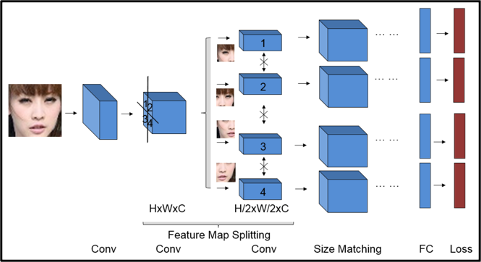
\includegraphics[width=1.0\textwidth]{image2-23-a}
  \caption{ }
  \label{image2-23-a}
\end{subfigure}
\begin{subfigure}{.5\textwidth}
  \centering
  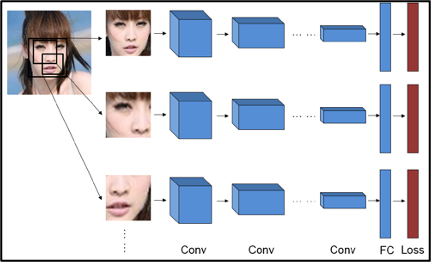
\includegraphics[width=1.0\textwidth]{image2-23-b}
  \caption{ }
  \label{image2-23-b}
\end{subfigure}
  \caption{ (آ) شبکه عصبی پیچشی \lr{SplitNet}  (ب) شبکه عصبی پیچشی معمولی \cite{WEN201894}.}
\label{image2-23}
\end{figure}

\subsubsection{	شبکه \lr{GoogLeNet}}
در سال 2015 \lr{Christian Szegedy} و همکاران \cite{7298594} یک شبکه عصبی عمیق به نام \lr{GoogLeNet} ارائه دادند. همانطور که در شکل \ref{image2-24} مشاهده می‌شود، \lr{GoogLeNet} یک شبکه عصبی پیچشی با 22 لایه است که یکی از اولین معماری های شبکه عصبی پیچشی بود که از رویکرد کلی قرار دادن تعداد زیادی از لایه‌های پیچشی و رای گیری  در کنار هم در یک ساختار متوالی بدست آمد. نویسندگان این مقاله همچنین تأکید کردند که این مدل جدید، توجه قابل ملاحظه ای به مصرف حافظه و مصرف انرژی دارد، زیرا کنار هم چیدن تعداد زیادی لایه و فیلتر دارای هزینه محاسباتی و حافظه است که احتمال بیش‌برازش  را افزایش می‌دهد.
 
\begin{figure}[h]
\centering
  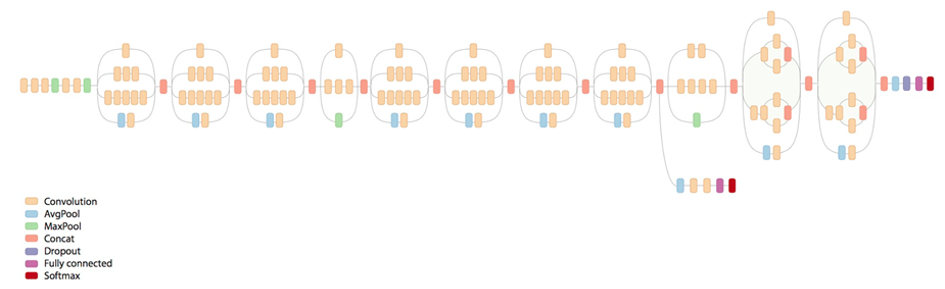
\includegraphics[width=1.0\textwidth]{image2-24}
  \caption{معماری کلی شبکه \lr{GoogLeNet} \cite{7298594}.}
  \label{image2-24}
\end{figure}

\subsubsection{	شبکه \lr{VGGFace}}
در سال 2015 \lr{Omkar M. Parkhi} و همکاران \cite{parkhi2015deep} شبکه عمیق \lr{VGGFace} را ارائه کردند که شامل یک توالی طولانی از لایه‌های پیچشی می‌باشد. با توجه به شکل \ref{image2-27} این شبکه که در لایه آخر به عنوان یک طبقه‌بند عمل می‌نماید، هر تصویر آموزشی چهره را توسط لایه تماما متصل و تابع ضرر \lr{softmax log-loss} به یک بردار تبدیل می‌نماید که هر مقدار در این بردار، نشان دهنده احتمال برای یک هویت فردی است. \lr{VGGFace} مشابه \lr{FaceNet} از یک تابع ضرر سه گانه \LTRfootnote{Triplet Loss Function} در آموزش برای بهبود عملکرد کلی استفاده می‌نماید.
 
\begin{figure}[h]
\centering
  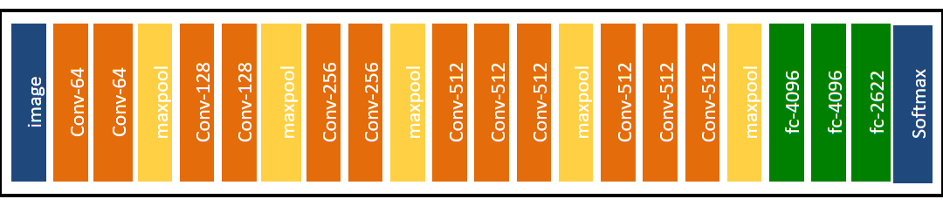
\includegraphics[width=1.0\textwidth]{image2-27}
  \caption{معماری شبکه \lr{VGGFace} \cite{parkhi2015deep}.}
  \label{image2-27}
\end{figure}

\subsubsection{نقاط راهنما} 
چهره‌هایى كه در جهت‌هاى مختلفى هستند، براى سامانه تشخیص چهره، متفاوت به نظر می‌رسند. براى غلبه بر این چالش در رویکردهای مبتنی بر نقاط راهنما سعى می‌شود تصویر را چرخانده و جابه جا نمود، بطوریكه چشم‌ها و لب‌ها در یك موقعیت خاص در تصویر قرار بگیرند. بدین ترتیب مقایسه چهره‌ها در مرحله بعد بسیار ساده‌تر خواهد شد.

\noindent 
در سال 2014 وحید كاظمى و جوزفین سالیوان در \cite{6909637} یک الگوریتم برای یافتن نقاط راهنما \LTRfootnote{Landmark} بر روی چهره ارائه دادند كه از 194 نقطه خاص كه در هر چهره اى وجود دارد استفاده می‌نماید. شکل \ref{image2-28} مکان این نقاط را بر روی گونه، لبه-هاى بیرونی چشم، كناره ابرو و... نشان می‌دهد. سپس این 194 نقطه به سامانه آموزش داده می‌شود تا در هر چهره‌اى آن-ها را تشخیص دهد. 
\begin{figure}[h]
\centering
  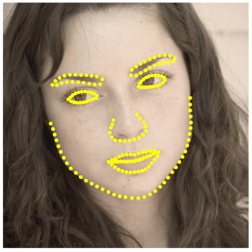
\includegraphics[scale=1]{image2-28}
  \caption{نتیجه موقعیت 194 شاخص روی چهره \cite{6909637}.}
  \label{image2-28}
\end{figure}

\noindent
پس از این که دانستیم چشم‌ها، دهان و ... کجاست، به راحتی می‌توانیم تناسب تصویر را تغییر داده و آن را چرخانده یا برش بزنیم. به طوری که چشم‌ها و دهان در بهترین حالت ممکن در مرکز قرار گیرد. با استفاده از تغییرات اساسی و اصلی تصویر، مانند تغییر اندازه، چرخش، خطوط موازی را حفظ می‌کنیم که در ریاضی به آن تغییرات نسبت یا افاین می‌گویند. شکل \ref{image2-29} علامت گذاری تکراری خطوط راهنما بر روی چهره را نشان می‌دهد. 
\begin{figure}[h]
\centering
  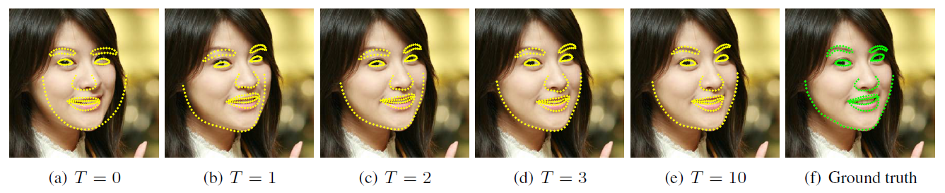
\includegraphics[width=1.0\textwidth]{image2-29}
  \caption{علامت گذاری خطوط راهنما بر روی چهره که در هر تکرار با کاهش خطا همراه می باشد \cite{6909637}.}
  \label{image2-29}
\end{figure}

\noindent
در سال 2016 \lr{Yue Wu} و همکاران \cite{wu2016facial} رویکردی برای یافتن نقاط راهنما بر روی چهره مبتنی بر شبکه عصبی پیچشی ارائه دادند. در این مقاله یک معماری جدید برای شبکه عصبی پیچشی به نام \lr{Tweaked CNN} پیشنهاد شده است که به اختصار \lr{TCNN} نامیده می‌شود. این شبکه عصبی عمیق از 4 لایه پیچشی ($CL_1 \dots CL_4$) با لایه‌های رای‌گیری در میان آن‌ها تشکیل شده است و در انتهای یک لایه تمام متصل  $FC_5$ و پس از آن یک لایه خروجی با اندازه $2*m$ آمده است که مختصات m نقطه ویژه را بر روی چهره مشخص می‌کند. در این مقاله m برابر با 5 در نظر گرفته شده است. تابع فعالیت برای هریک از لایه‌های پیچشی $f(x)=|tanh⁡(x)|$ و تابع فعالیت برای لایه تمام متصل $f(x)=tanh⁡(x)$ در نظر گرفته شده است. و در نهایت رابطه \ref{eq2-12} به عنوان تابع ضرر معرفی شده است.

\begin{equation}\label{eq2-12}
L(P_i,\hat{P_i})=\frac{(‖P_i-P ̂_i ‖_2^2)}{(‖P ̂_(i,1)-P ̂_(i,2) ‖_2^2 )}	
\end{equation}

\noindent
که در آن $P_i$ یک بردار $2*m$ برای مختصات پیش بینی شده تصویر $I_i$ و $P_i$ و مختصات محل دقیق آن نقاط می‌باشد. $P_{i,1}$ و $P_{i,2}$ مختصات چشم ها در تصویر مرجع می‌باشند. در نهایت خروجی لایه تمام متصل توسط الگوریتم \lr{GMM} به 64 خوشه تقسیم شده و هریک به صورت جداگانه بررسی شده است. معماری \lr{TCNN} در شکل \ref{image2-30} قابل مشاهده می‌باشد. این شبکه برای آموزش از مجموعه داده \lr{LFW} استفاده کرده است.

\begin{figure}[h]
\centering
  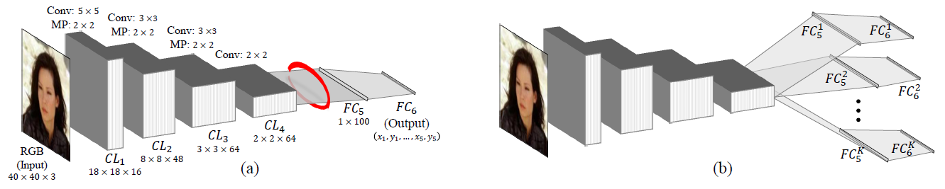
\includegraphics[scale=1]{image2-30}
  \caption{ شبکه عصبی پیچشی با معماری \lr{TCNN} \cite{wu2016facial}.}
  \label{image2-30}
\end{figure}

\subsubsection{\lr{OpenFace}}
در سال 2016، \lr{Amos} و همکاران \cite{amos2016openface} یک روش شناسایی چهره به نام \lr{OpenFace} ارائه دادند که ویژگی اصلی آن، آموزش شبکه عصبی عمیق در کمترین زمان و قابلیت اجرا بر روی دستگاه های قابل حمل مانند تلفن همراه با در نظر گرفتن منابع محدود می‌باشد. یک تصویر شامل تعدادی چهره به الگوریتم داده می‌شود. پس از یافتن چهره‌ها و مجزا کردن \LTRfootnote{Isolate} آن‌ها از یکدیگر، هر چهره به طور جداگانه مورد پیش پردازش \LTRfootnote{Preprocessing} قرار می گیرد و حجم آن کاهش می یابد. کاهش حجم تصویر برای عملکرد مناسب یک طبقه بندی بهینه بسیار مهم می‌باشد. تصاویر چهره ها باید هنجارسازی شده و ابعاد آن ها ثابت گردد تا به بخش شناسایی چهره راه یابند. هر تصویر چهره باید مورد تبدیل قرار بگیرد تا چشم ها، بینی و دهان، در مکان مشخصی قرار گیرند. بدین منظور از یک تبدیل هم نسبی \LTRfootnote{Affine Transformation} دوبعدی ساده استفاده می گردد. ابتدا باید چهره توسط 68 نقطه ویژه، نشانه گذاری شود. سپس نشانه های اطراف چشم ها و بینی (شکل \ref{image3-2}) برای محاسبه عامل های تبدیل هم نسبی استفاده می‌شوند. پس از انجام تبدیل هم نسبی، تصاویر چهره برش زده شده و اندازه آن ها 96×96 پیکسل می‌شود.

\begin{figure}[h]
	\centering
	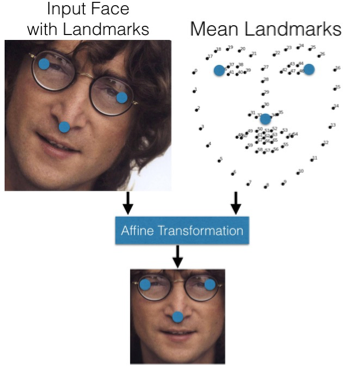
\includegraphics[scale=1]{image3-2}
	\caption{
		تبدیل هم نسبی \lr{OpenFace} براساس نقاط ویژه آبی  
		\cite{amos2016openface}.}
	\label{image3-2}
\end{figure}

\noindent‏ 
پس از پیش پردازش، تصاویر چهره ها به عنوان ورودی به یک شبکه عصبی پیچشی داده می‌شوند (شکل \ref{image3-3}). این الگوریتم برای تعلیم شبکه از مجموعه داده کوچکی با 500 هزار تصویر چهره استفاده می کند که از ادغام دو مجموعه داده بزرگ برچسب گذاری شده به نام \lr{CASIA-WebFace} و \lr{FaceScrub} بدست آمده است. شبکه مورد استفاده در این الگوریتم یک نسخه اصلاح شده از شبکه \lr{nn4} الگوریتم \lr{FaceNet} می‌باشد. شبکه \lr{nn4} مبتنی بر معماری \lr{GoogLeNet} می‌باشد. برای تعیین میزان شباهت نتیجه، از فاصله اقلیدسی استفاده شده است.
\begin{figure}[h]
	\centering
	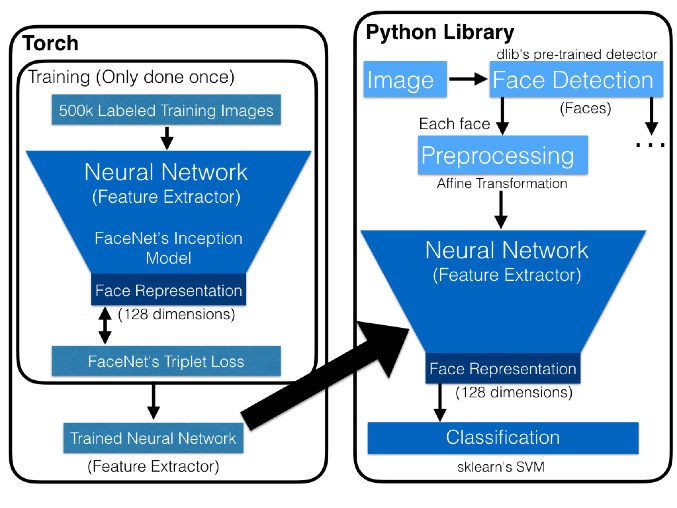
\includegraphics[scale=1]{image3-3}
	\caption{معماری \lr{OpenFace}  \cite{amos2016openface}.}
	\label{image3-3}
\end{figure}

\noindent
هر تصویر از یک شبکه یکتا به یک سه گانه نگاشت داده می‌شود. گرادیان خطای سه گانه برای هر تصویر محاسبه شده و پس‌انتشار خطا صورت می‌پذیرد. در هر دسته کوچک\LTRfootnote{Mini Batch}، \lr{P} تصویر برای هر نفر از \lr{Q} نفر، در مجموعه داده انتخاب می‌شود. سپس $M \approx PQ$ تصویر به شبکه داده می‌شود تا عملیات رو به جلو \LTRfootnote{forward} انجام پذیرد. در این مقاله از $P=20$ و $Q=15$ استفاده شده است. تمام جفت های لنگر-مثبت برای بدست آوردن سه گانه های $N = Q \binom{P}{2}$ مورد استفاده قرار می‌گیرند. خطای سه گانه محاسبه شده و مشتق آن برای پس انتشار خطا استفاده می‌شود. شکل \ref{image3-4} چگونگی آموزش شبکه را نشان می‌دهد.

\begin{figure}[h]
	\centering
	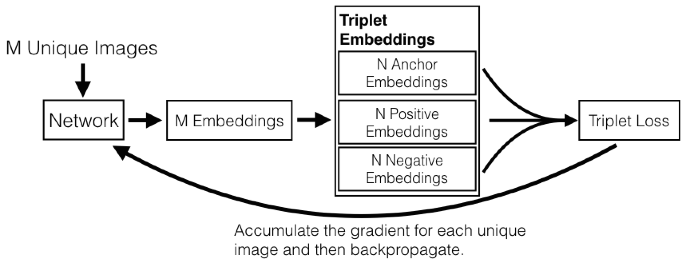
\includegraphics[scale=1]{image3-4}
	\caption{جریان یادگیری در معماری \lr{OpenFace} \cite{amos2016openface}.}
	\label{image3-4}
\end{figure}

\noindent
مجموعه داده \lr{LFW} یک معیار استاندارد برای سنجیدن میزان دقت الگوریتم های تشخیص چهره می‌باشد. الگوریتم \lr{OpenFace} بر روی این مجموعه داده مورد سنجش قرار گرفت که به دقت
$0.9292 \pm 0.0134 \%$ 
رسید.

\subsubsection{	شبکه \lr{MobileNet}}
در سال‌های بعد شبکه‌های عمیق‌تر، پهن‌تر و البته پیچیده‌تر مانند \lr{GoogleNet}  و \lr{ResNext}، \lr{ResNet} برای رسیدن به دقت بالاتر مطرح شد. با وجود پیچیدگی در طراحی این شبکه‌ها، تمرکز اصلی ‌بر روی دقت بود و جای خالی شبکه‌های با سایز کوچک و سرعت بالا با قابلیت استفاده در رباتیک، بردهای مینی‌کامپیوتری و البته موبایل‌ها احساس می‌شد که ایده دسته جدیدی از شبکه‌های کانولوشنی سبک با پارامترهای کم‌ شکل گرفت. 

\noindent
یکی از شاخص‌ترین شبکه‌های سبک، شبکه عصبی MobileNet نام دارد که توسط محققان گوگل \cite{howard2017mobilenets} با هدف طراحی شبکه‌های کارآمد، سبک، سریع و با دقت قابل‌قبول مطرح شده است. در این مقاله یک نوع کانولوشن جدید به‌نام کانولوشن \LTRfootnote{Depth-Wise Separable convolution} \lr{DWS} معرفی شد که قلب تپنده شبکه موبایل نت است. در کانولوشن DWS ابتدا کانولوشن عمقی اعمال می‌شود و سپس کانولوشن نقطه‌ای که به‌ترتیب نقش مراحل فیلتر و ادغام در کانولوشن استاندارد را دارند. 

\noindent
در کانولوشن استاندارد M کرنل $k \times k$ داشتیم. اما در اینجا تنها یک کرنل $k \times k$ داریم. با این کرنل، مرحله اول کانولوشن را انجام می‌دهیم. با انجام عمل فیلتر، هر صفحه از کرنل در یک صفحه از نقشه ویژگی ورودی F کانوالو می‌شود. به این مرحله کانولوشن عمقی گفته می‌شود.  مرحله دوم، کانولوشن نقطه‌ای \LTRfootnote{point-wise} است. این مرحله معادل با مرحله ادغام در کانولوشن استاندارد است. اما یک تفاوت اساسی بین مرحله ادغام در کانولوشن استاندارد و کانولوشن DWS این است که مرحله ادغام در کانولوشن استاندارد، یک جمع ساده است، اما مرحله ادغام در کانولوشن DWS شامل یک کانولوشن 1×1 است. کانولوشن نقطه‌ای همان کانولوشن استاندارد یا رایجی هست که می‌شناسیم و در بسیاری از شبکه‌های کانولوشنی استفاده می‌شود. این کانولوشن 1×1 وظیفه مهمی دارد و خروجی‌های کانولوشن عمقی (مرحله اول) را با هم ادغام می‌کند. در مرحله قبل بجای تعریف M کرنل، تنها یک کرنل تعریف کردیم. اما در این مرحله، M کرنل 1×1 تعریف می‌کنیم.

\begin{figure}[h]
\centering
  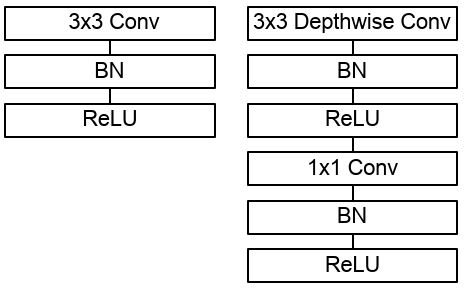
\includegraphics[scale=0.5]{image2-31}
  \caption{
  کانولوشن DWS که شامل دو کانولوشن depth-wise و point-wise است. 
   \cite{howard2017mobilenets}.}
  \label{image2-31}
\end{figure}

\noindent
شبکه عصبی موبایل نت 4.2 میلیون پارامتر دارد. وقتی تعداد پارامترهای این شبکه را با شبکه محبوب ResNet-18 با 11 میلیون پارامتر مقایسه کنیم، متوجه می‌شویم که چقدر میزان پارامترها کمتر است. این مقایسه در جدول \ref{tbl2-2} قابل مشاهده می‌باشد.

\begin{table}
\centering
  \caption{ مقایسه شبکه عصبی موبایل نت با گوگل نت و VGG.}
  \label{tbl2-2}
  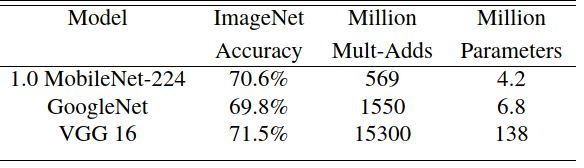
\includegraphics[width=0.5\textwidth]{table2-2}
\end{table}

\noindent
در سال ۲۰۱۹  \lr{Andrew Howard} و همکاران \cite{howard2019searching} معماری \lr{MobileNet} نسخه ۳ را ارائه دادند. در این معماری مسیر استخراج ویژگی از ۴ لایه كانولوشن، ۱ لایه رای گیری، ۱۵ لایه تنگنا \LTRfootnote{Bottleneck}  و ۸ ماژول توجه \LTRfootnote{Attention} تشکیل شده است، تصویر ورودی به بخش استخراج ویژگی داده می‌شود و مدل در این مسیر به طور خودكار یك سلسله مراتب ویژگی را از تصاویر ورودی آموزش خواهد دید و در نهایت این ویژگی‌های استخراج شده به عنوان ورودی دسته بند مورد استفاده قرار می‌گیرد. ایده اصلی این مقاله استفاده از بلاک‌های \lr{ Squeeze-and-Excite} می‌باشد. معماری \lr{MobileNet} نسخه ۳ در شکل \ref{image2-32} قابل مشاهده می‌باشد. 

\begin{figure}[h]
\centering
  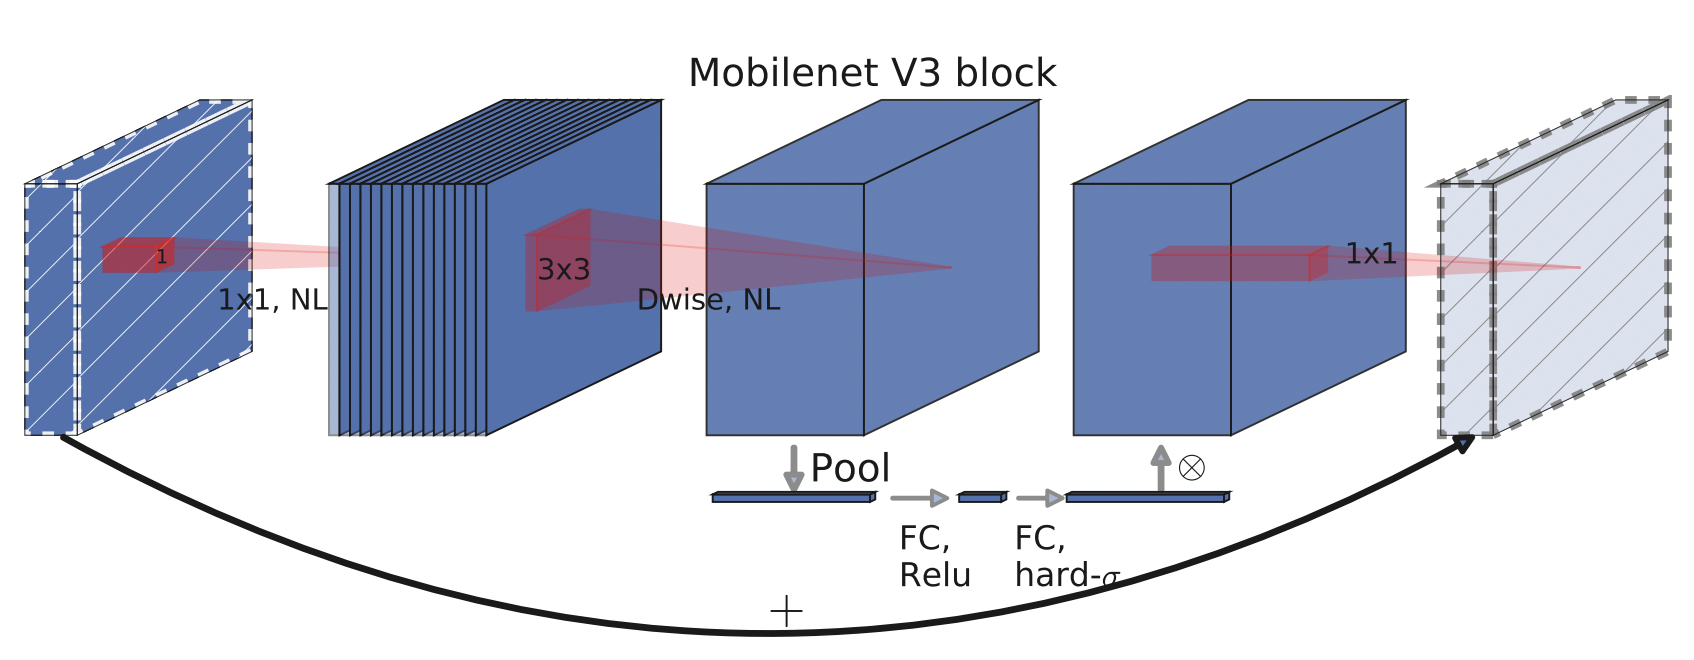
\includegraphics[width=1\textwidth]{image2-32}
  \caption{
لایه‌های MobileNet به همراه ماژول‌ \lr{ Squeeze-and-Excite} که در بخش پایین سمت چپ قابل مشاهده می‌باشد 
   \cite{yang2021sanet}.}
  \label{image2-32}
\end{figure}

\subsubsection{لایه توجه}
در سال ۲۰۲۱ yang و همکاران \cite{yang2021sanet} یک ماژول مبتنی بر لایه توجه ارائه دادند. لایه‌های توجه که یک شبکه عصبی را قادر می‌سازد تا دقیقاً بر روی عناصر مهم مربوط به ورودی متمرکز شود، به یک جز اساسی برای بهبود عملکرد شبکه‌های عصبی عمیق تبدیل شده است. عمدتا دو مکانیسم توجه به طور گسترده در بینایی رایانه مورد استفاده قرار می گیرد: لایه توجه وابسته به كانال \LTRfootnote{Channel Attention Module} و لایه توجه وابسته به موقعیت \LTRfootnote{Spatial Attention Module} که به ترتیب به منظور توجه به رابطه دو به دو در سطح کانال و در سطح پیکسل هستند. اگرچه تلفیق آن‌ها ممکن است عملکرد بهتری نسبت به پیاده سازی های منفرد آنها به دست آورد‌، اما سربار محاسباتی را افزایش می‌دهد.

\noindent
در این مقاله، یک ماژول \lr{Shuffle Attention} کارآمد با محاسباتی کم پیشنهاد شده است که آن را به اختصار ماژول \lr{SA} می‌نامیم. ابتدا ابعاد کانال را به چندین ویژگی فرعی قبل از پردازش موازی آنها تقسیم می‌کند. سپس، برای هر زیر‌ویژگی از یک واحد Shuffle برای به تصویر کشیدن وابستگی‌های ویژگی در هر دو بعد مکانی و کانال استفاده می‌کند. پس از آن ، همه زیر‌ویژگی‌ها جمع می‌شوند و یک عملگر تغییر کانال برای امکان برقراری ارتباط اطلاعاتی بین ویژگی‌های فرعی مختلف به کار گرفته می‌شود. معماری این ماژول در شکل \ref{image2-33} آمده است.

\begin{figure}[h]
\centering
  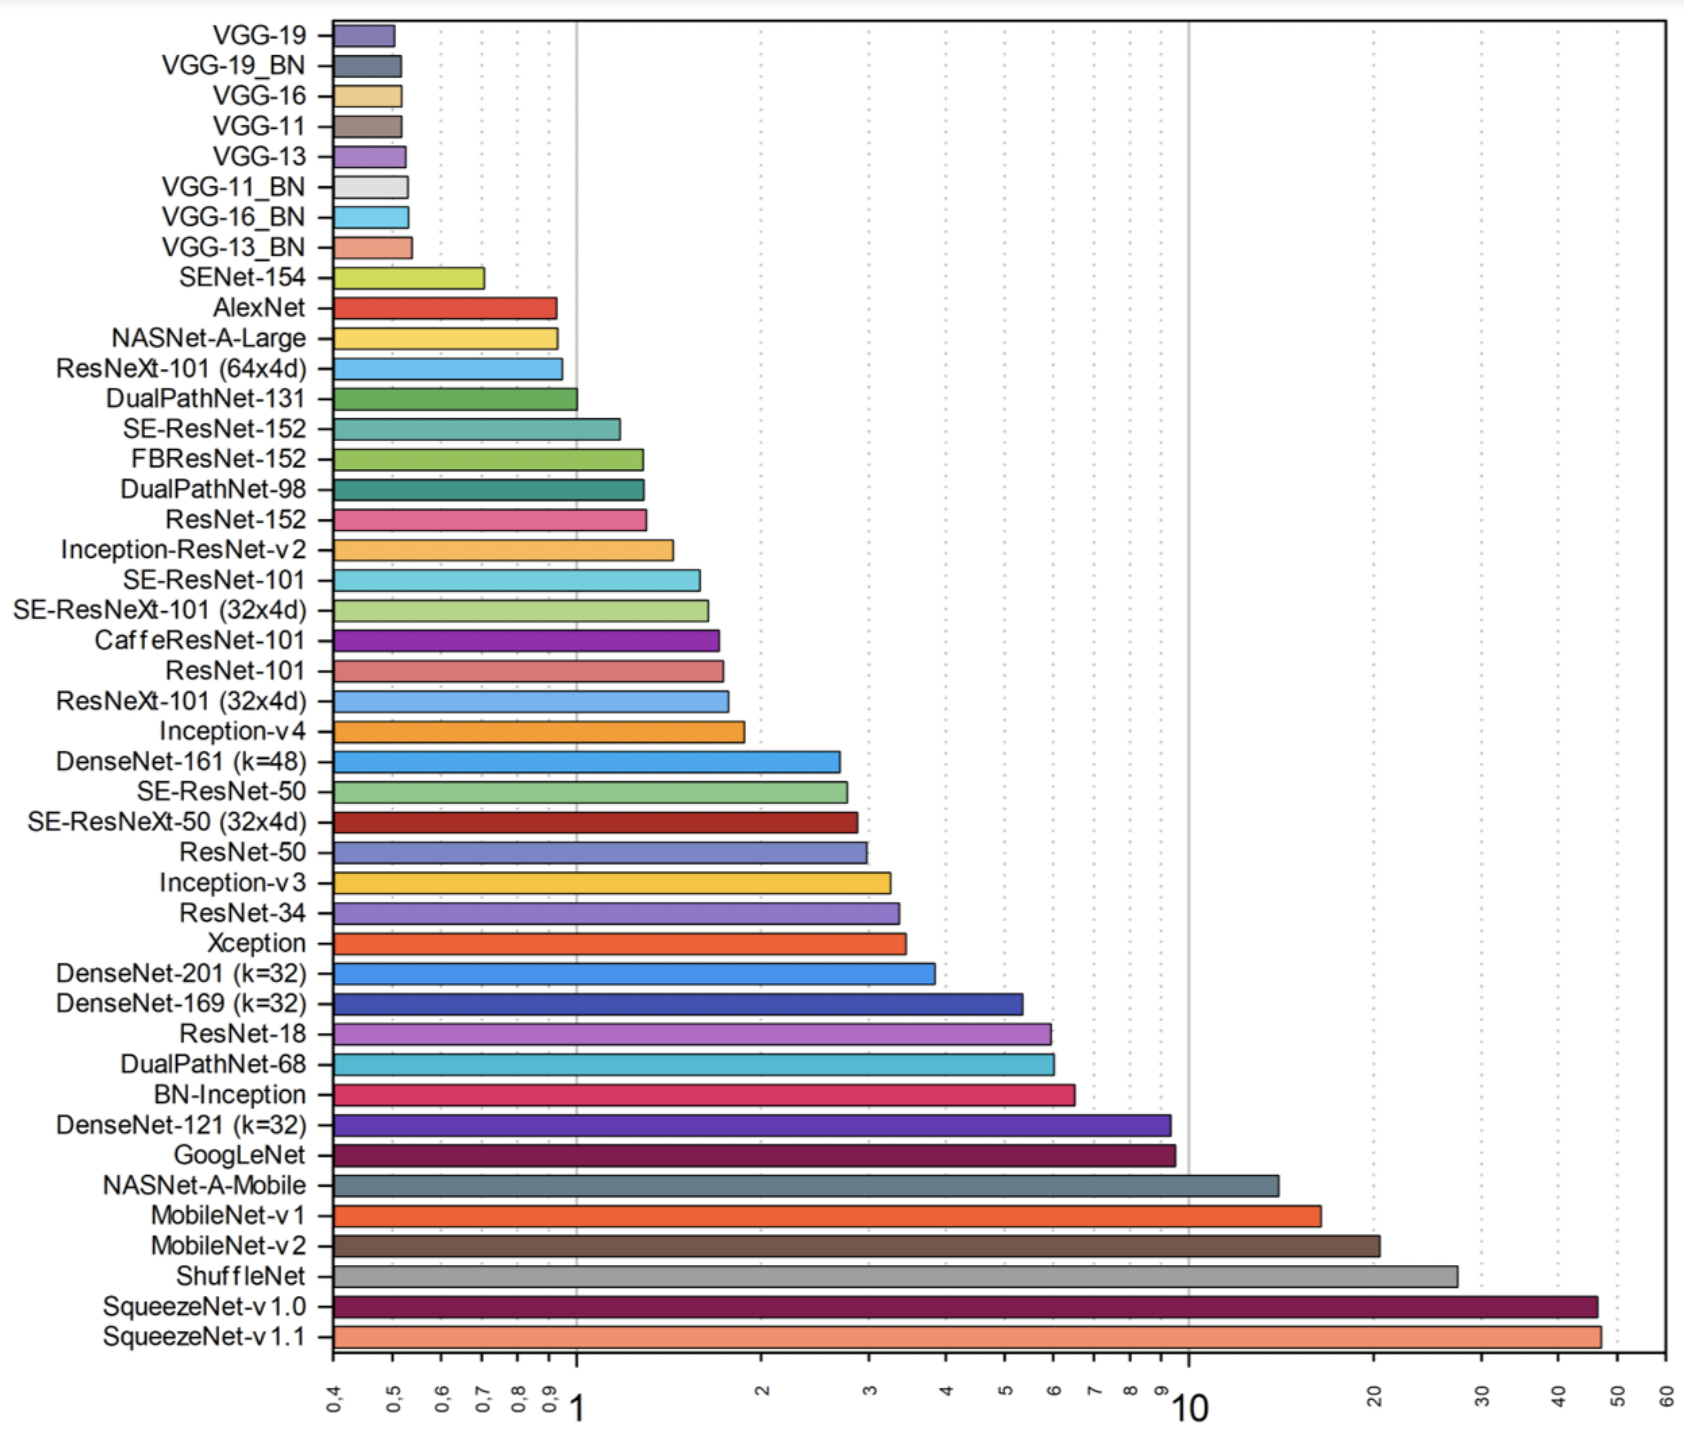
\includegraphics[width=1\textwidth]{image2-33}
  \caption{
  معماری ماژول \lr{Shuffle Attention}
   \cite{yang2021sanet}.}
  \label{image2-33}
\end{figure}

\noindent
پارامترها و محاسبات SA در شبکه ResNet50 به ترتیب 300 در مقابل 25.56 میلیون است، اما افزایش عملکرد بیش از ۱٫۳۴٪ را به ارمغان می‌آورد. نتایج تجربی نشان می‌دهد که SA برای دستیابی به دقت بالاتر مناسب است، در حالی که دارای پیچیدگی مدل کمتری است و از روش های جدید \LTRfootnote{State of the Art} کنونی به مراتب بهتر عمل می‌کند.

\section{نتیجه گیری}
در این فصل مفاهیم‌ پایه در مبحث یافتن و تشخیص چهره در تصاویر و انواع الگوریتم‌های دسته‌‌بندی از روی تصاویر رنگی بررسی شد. سپس به طور مخصوص به معماری‌های مطرح شبکه‌های یادگیری عمیق در زمینه دسته‌بندی چهره پرداخته شد. نتایج بررسی به طور خلاصه در شکل \ref{image2-34} مشاهده می‌شود. 

\begin{figure}[h]
	\centering
	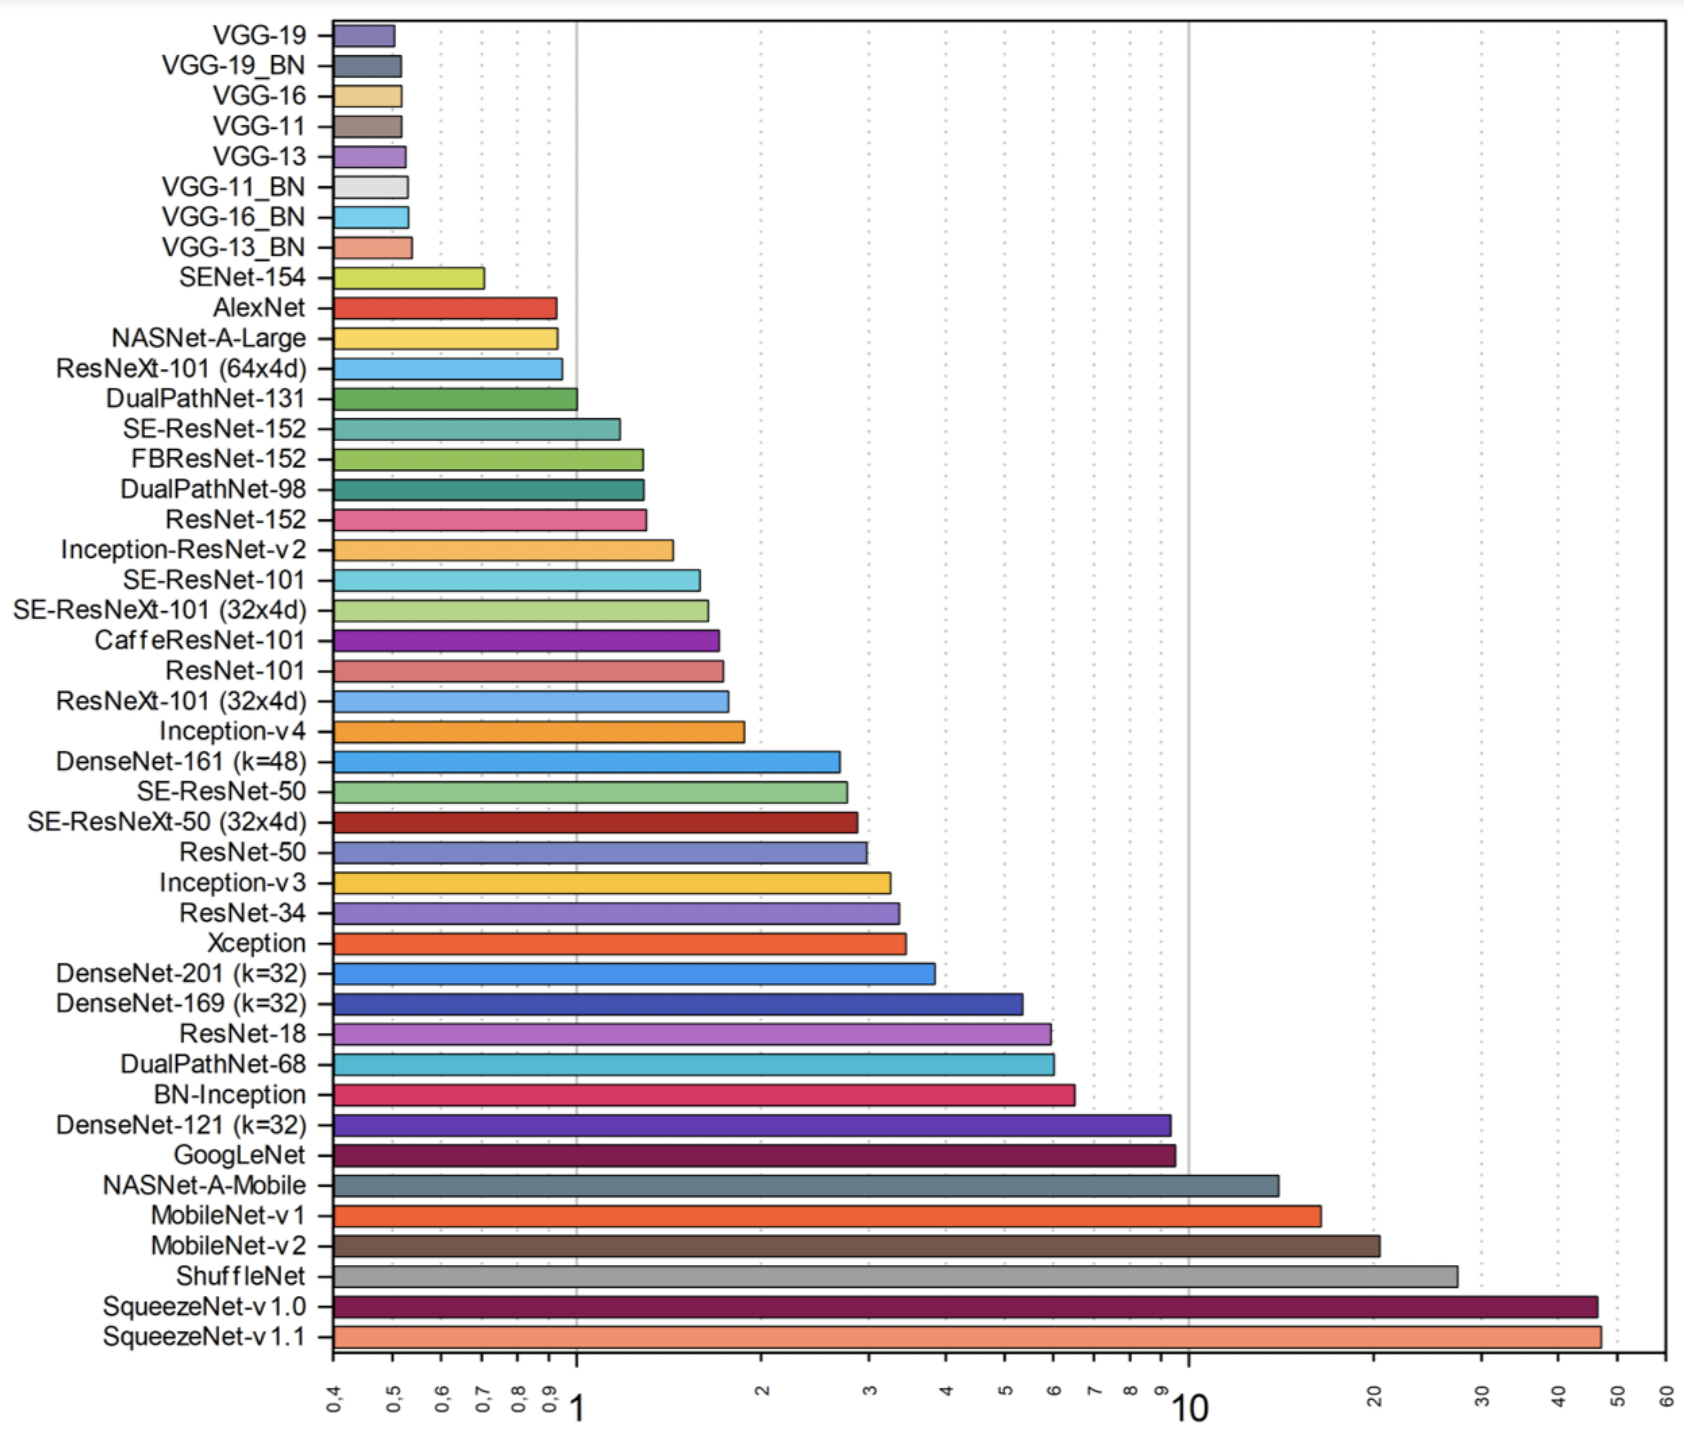
\includegraphics[width=0.75\textwidth]{image2-34}
	\caption{
		مقایسه چگالی دقت در معماری‌های مختلف شبکه عصبی پیچشی 
		\cite{Bianco_2018}.}
	\label{image2-34}
\end{figure}

\noindent
همان طور که در شکل در شکل \ref{image2-34} آمده است، با بررسی شبکه‌های به‌روز از جمله
\lr{EfficientNetB0} ،
\lr{ResNet-50} ،
\lr{VGG19} ،
\lr{SqueezeNet} ،
\lr{MobileNet}
و
\lr{MobileNetV2}
و مقایسه دقت و زمان پاسخگویی آن‌ها، به این نتیجه می‌رسیم که شبکه‌های \lr{MobileNetV2} و \lr{SqueezeNet} دارای چگالی دقت بالاتری می‌باشند. بدین معنا که نسبت دقت دسته بندی به تعداد پارامترهای شبکه در آن‌ها بیشتر می‌باشد. بنابرین می‌توان سرعت اجرای مناسب و همچنین دقت مناسب را از آن‌ها انتظار داشت. 

